\documentclass[a4paper,twoside]{article}
\usepackage{listings}
\usepackage{xcolor}
\usepackage{url}
\usepackage{changepage}
\usepackage{graphicx}
\usepackage[hungarian]{babel}
\usepackage{amsmath} 
\usepackage{t1enc}
\usepackage{titlesec}
\usepackage{placeins}
\title{Szakdolgozat}

\definecolor{mygreen}{RGB}{0,128,0}
\definecolor{mygray}{RGB}{204,255,153}
\definecolor{mymauve}{RGB}{204,102,0}
\definecolor{myblue}{RGB}{0,0,204}
\definecolor{mypurple}{RGB}{204,0,204}

\graphicspath{{./images}}
\author{Bozsik József}

\lstdefinestyle{javascriptStyle}{
	language=Python,  % Change this to JavaScript
	basicstyle=\ttfamily,  % Keyword style for the second keyword list
	commentstyle=\color{mygreen},
	stringstyle=\color{mymauve},
	numberstyle=\tiny\color{mygray},
	numbers=left,
	stepnumber=1,
	numbersep=10pt,
	backgroundcolor=\color{white},
	frame=single,
	rulecolor=\color{black},
	showspaces=false,
	showstringspaces=false,
	showtabs=false,
	tabsize=2,
	captionpos=b,
	frame=none,
	breaklines=true,
	morekeywords=[1]{let, const, async, var, function, return, else, for, while, section},
	keywordstyle=[1]\color{myblue}, % Use keywordstyle1 for the first set of keywords
	morekeywords=[2]{if,await,},
	keywordstyle=[2]\color{mypurple}, % Use keywordstyle2 for the second set of keywords  % Add 'await' to the morekeywords list
	escapeinside={(*@}{@*)},
	xleftmargin=0pt,
	xrightmargin=0pt,
}

\begin{document}
\maketitle
\newpage
\tableofcontents
\newpage
{
\section*{Hallgatói nyilatkozat}}
Alulírott \textit{Bozsik József}, szigorló hallgató kijelentem, hogy ezt a szakdolgozatot meg
nem engedett segítség nélkül, saját magam készítettem, csak a megadott forrásokat (szakirodalom, eszközök stb\ldots) használtam fel. Minden olyan részt, melyet szó szerint, vagy
azonos értelemben, de átfogalmazva más forrásból átvettem, egyértelműen, a forrás megadásával megjelöltem.
Hozzájárulok, hogy a jelen munkám alapadatait (szerző(k), cím, angol és magyar
nyelvű tartalmi kivonat, készítés éve, konzulens(ek) neve) a BME VIK nyilvánosan hozzáférhető elektronikus formában, a munka teljes szövegét pedig az egyetem belső hálózatán
keresztül (vagy autentikált felhasználók számára) közzétegye. Kijelentem, hogy a benyújtott munka és annak elektronikus verziója megegyezik. Dékáni engedéllyel titkosított diplomatervek esetén a dolgozat szövege csak 3 év eltelte után válik hozzáférhetővé.
\begin{flushleft}
	Budapest, 2022. december 6.
\end{flushleft}

\newpage
\section{Összefoglaló}
A szakdolgozat témájaként egy társasjáték készítését választottam webes környezetben mivel személy szerint mindig is érdekelt a teljes web-fejlesztési folyamat, valamint egyik kedvenc időtöltéseim közé tartozik a barátokkal egy közös társasjátékozás. 
Végül egy ''ki nevet a végén'' társas fejlesztése mellett döntöttem, hiszen a szabályok nem túl bonyolultak, viszont sok lehetőség van kreatívnak lenni az implementálás során, valamint inspirálódni is lehet az eddig elkészült játékokból amik az interneten megtalálhatók.

Társasjáték lévén, a játékot több felhasználó is játszhatja egyszerre.  Az interneten rengeteg olyan web-alkalmazás van, ahol hasonló társasjátékkal
lehet játszani, viszont a belépés nehézkes, a játék kezelése bonyolult. A célom az volt, hogy
egy letisztult felületen könnyedén és egyszerűen lehessen élvezni a társasjáték adta
élvezeteket a partnereinkkel.

Ebben a dokumentumban összefoglalom, hogy hogyan implementáltam, mind a szerveroldali,
mind a kliensoldali szoftvert. Az alkalmazás készítése során rengeteg újfajta technológiát és
keretrendszert használtam, amik jól bevált eszközök a webfejlesztésben. A munkahelyem
által biztosított szervert is használtam a megvalósításához, ami a játék logikáját biztosította. A
végeredmény egy egyszerű, és könnyen kezelhető webalkalmazás lett, ami kis
továbbfejlesztéssel versenytársa lehet az interneten található játékoknak.


\newpage
\section{Abstract}
As the topic of my thesis, I chose to create a board game in a web environment. Personally, I've always been interested in the entire web development process, and one of my favorite pastimes is playing board games with friends. Ultimately, I decided to develop a "Who Laughs Last" board game because the rules are not overly complicated, offering ample room for creativity during implementation, as well as inspiration from existing online games.

Given that it's a board game, multiple users can play it simultaneously. While there are many web applications offering similar board games online, the entry process can be cumbersome, and game management can be complex. My goal was to provide a clean interface for easily enjoying the board game with partners.

In this document, I summarize how I implemented both the server-side and client-side software. Throughout the application development, I utilized various new technologies and frameworks, proven tools in web development. I also used a server provided by my workplace to support the game's logic. The end result is a simple and user-friendly web application that, with some further development, could become a competitor to existing online games.
\newpage
\section{Bevezetés}
A webfejlesztés a mindennapi internetes böngészés során használt weboldalak és
webalkalmazások létrehozásának folyamata. Amikor egy weboldalt látogatunk, például
közösségi média platformokat, online vásárlási oldalakat vagy hírportálokat, akkor a
webfejlesztés végtermékét látjuk.
A weboldalakat programozási nyelvek, keretrendszerek és eszközök kombinációjával építik
fel. A webfejlesztés két fő komponense a frontend és a backend.
A frontend az, amit egy weboldalon látunk és amivel interakcióba lépünk. Ide tartozik az
oldal tervezése, elrendezése és felhasználói felülete, valamint a felhasználói inputok
ellenőrzése is. A frontend létrehozásához a fejlesztők olyan nyelveket használnak, mint az
HTML\footnote{Hypertext Markup Language}, CSS\footnote{Cascading Style Sheets} és a JavaScript. Az
HTML strukturálja a weboldal tartalmát, a CSS pedig esztétikus megjelenést biztosít, míg a
JavaScript interaktivitást és funkcionalitást ad hozzá.
A backend felelős a weboldal háttérlogikájáért és feldolgozásáért. Feladatokat lát el, mint az
adatok tárolása és lekérdezése, felhasználói azonosítás és a szerverkommunikáció. A
fejlesztők különböző programozási nyelveket és keretrendszereket, például az én esetemben
Java Spring\cite{javaspring}-re esett a választás mivel a munkahelyemen ezt a környezetet használják a
backend létrehozásához. Emellett adatbázisokkal kommunikálnak az információ tárolásához
és lekérdezéséhez. Az én implementációmban az utóbbi nem történt meg, hiszen a
munkahelyem által biztosított szerveren tároltam az adatokat.
A webfejlesztés gyakran API\footnote{Application Programming Interface} hívásokat tartalmaz más
szerverek felé adatok lekéréséhez vagy specifikus műveletek végrehajtásához. Ezek az API
hívások lehetővé teszik a különböző rendszerek közötti kommunikációt és információcsere
zavartalan működését. Közismert hasonlat az API-ra, hogyha egy étteremben a konyha
részleg a backend, az asztalok a frontend, ahol a vendégek (felhasználók) ülnek, akkor az API
a pincér, aki kézbesíti az ételt (adatokat).
A következő fejezetekben ismertetem, hogy az alábbi technológiákat miként valósítottam
meg, és milyen keretrendszereket használtam, amik a fejlesztést, és a felhasználói élményt is
egyaránt segítik.
\newpage

\section{Feladatkiírás pontosítása és részletes elemzése}
Magát a feladatot a külső konzulensem adta meg és specifikálta, hogy mire kell hogy képes
legyen az alkalmazás, valamint milyen technológiákat használjunk. Maga az implementációt
teljesen rám bízta, hogy milyen osztályokat valósítok meg, azokat hogyan csoportosítom és
hogy hogyan dolgoznak együtt.
A ki nevet a végén társas szabályai vannak érvényben. Tehát egy játékos bábuja csak akkor
tud belépni a táblára, ha 6-ost dob. Ha viszont 6-ost dob valaki, akkor utána még egyszer
dobhat. Ha egy bábu ugyan arra a mezőre lép, ahol már éppen áll egy bábu, akkor leüti a
pályáról. Az a játékos győz, aki leghamarabb, az összes bábuját körbeviszi a táblán.
Mivel a web alkalmazást egy munkahelyi környezetben valósítottam meg, ott már adva volt
egy szerver, ami lényegében egy adatbázis-szerverként funkcionált, valamint játék bizonyos
szintű logikája is már implementálva volt. Tehát az alkalmazás backendjének kommunikálnia
kellett ezzel a szerverrel és feldolgoznia a válaszokat. Erre RESTful API-ra kellett küldeni a
kéréseket. RESTful API egy architekturális stílus és koncepció, amely a webes szolgáltatások
tervezését és fejlesztését írja le. A REST\footnote{Representational State Transfer} alapelveit követve
a RESTful API egy szabványos módszert nyújt a kommunikációra kliensek és szerverek
között. Ezeket az adatokat felhasználva a backend tovább küldi a frontendnek, ahol ezeket
megjeleníti.
Az alkalmazás főoldalán megjelennek az eddig létrehozott táblák, valamint információk
ezekről (hány játékos lépett már be, mennyi a maximum létszám, elindult-e már a játék,
stb\ldots). 

Egyszerre akár több játékost is beállíthatunk. Ezután elindítjuk a pályát, ami átnavigál egy
újabb oldalra, ahol a tábla van megjelenítve. Egy adott táblának 3 státusza lehet: CREATED,
STARTED, FINISHED. A CREATED státuszban tudnak a játékosok belépni az adott pályára. A STARTED állapotban folyik a játék, és már nem lehet csatlakozni hozzá. A FINISHED státuszban valamilyen módon véget ért a játék. A kockadobás egy sima gomb, amit ha a
felhasználó megnyom, véletlenszerűen létrehoz egy számot 1-től 6-ig. Ezután rákattint a bábura amit mozgatni
szeretne, és az a megfelelő mennyiséggel előre lép a táblán. Ha éppen ellenfél játékosra lép,
leüti a tábláról. Ha az összes bábu beér akkor kiírja, hogy nyert az adott játékos és maga a
tábla átvált FINISHED státuszra.

\begin{figure}
	\caption{Egy játékmenet ábrazolása}
	\raggedleft 
	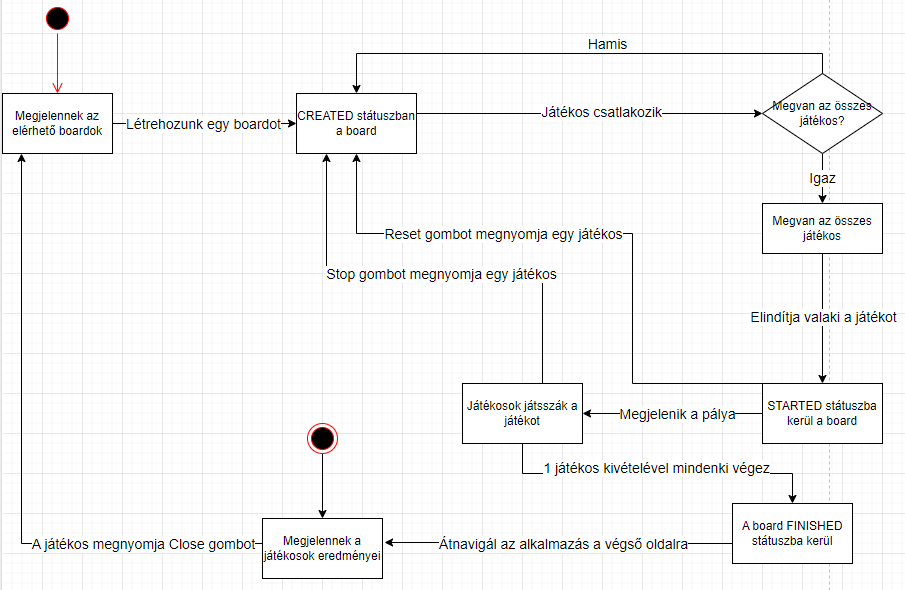
\includegraphics[scale=0.5]{folyamatabra}
	\label{folyamatabra}
\end{figure}
\newpage
\section{Alkalmazás fejlesztéséhez használt technológiák}
A modern webfejlesztésben szinte elengedhetetlen különböző keretrendszerek használata,
mivel a hatékonyságban, és a szoftverminőségben is jelentősen támogatja a munkájában a fejlesztőt.
\subsection{Frontend}

\subsubsection{Javascript keretrendszer}
Mivel az alkalmazásom felépítése több nézetből is állt, érdemes volt egy olyan keretrendszert választanom, ami támogatja a komponens 
alapú megközelítést. Ezt a  Vue.js\cite{vuejs} teljesíti is, így ezt a technológiát választottam. 

 A \textbf{komponens alapú architektúra} lényege, hogy már az egyszer megírt kódunkat többször, teljesen máshol is fel tudjuk használni. Például tipikus példa 
ha listázni akarunk valamiféle adatot, bizonyos formázások után. Erre létrehozhatunk egy komponenst amit többször megjelenítünk az oldalon, vagy esetleg teljesen máshol az alkalmazásunkban (\ref{komponens}.ábra).
\begin{figure}
	\caption{Board komponens listázása}
	\begin{minipage}{\textwidth}
		\begin{lstlisting}[style=javascriptStyle]
			<section>
			<Board data-test="board" v-for="board in boardStore.boards" :key="board.id" :board="board" />
			</section>
		\end{lstlisting}
	\end{minipage}
	\label{komponens}
\end{figure}
\FloatBarrier
A komponensen belül írjuk meg, hogy a komponens hogyan viselkedjen, függvényeket definiálhatunk bennük, eseménykezelőket hozhatunk létre, például egy gomb megnyomására mi történjen(\ref{button-click}.ábra). A komponensek egymásba ágyazhatóak így jöhet létre a szülő-gyermek viszony közöttük. Az ilyen komponensek között adatokat adhatunk át, valamint informálhatják különböző események bekövetkeztéről. 
\begin{figure}
	\caption{Egy gomb klikk eseménykezelőjének létrehozása}
	\begin{minipage}{\textwidth}
		\begin{lstlisting}[style=javascriptStyle]
		<button data-test="createButton" @click="creatingNewBoard = !creatingNewBoard"
		class="button is-primary"><font-awesome-icon style="margin-right: 3px;" :icon="['fas', 'plus']" />Create
		Board</button>
		\end{lstlisting}
	\end{minipage}
	\label{button-click}
\end{figure}

Mivel a társasjáték egy interaktív szórakozás, a felület sokszor fog változni, felhasználói input hatására. A letisztultság érdekében érdemes több kis komponenssel dolgozni, hiszen így az összetartózó felelősségek egy helyen vannak, ezáltal könnyebb őket változtatni, valamint bővíteni a kódbázist. Viszont a komponenseknek le kell tudniuk kezelni ha valamilyen input hatására, az általuk megjelenített adatok megváltoznak. Mindezt lekezelni nagyon nehéz lenne, viszont a Vue.js segít ebben. Számon tartja azokat az adatokat amiktől függnek az egyes komponensek és automatikusan frissíti őket, hogyha megváltoznak. Így tehát ha megfelelően osztjuk szét a komponensek felelősségeit, a felület csak azon része fog frissülni aminek muszáj, ezáltal az alkalmazásunk jól fog tudni skálázódni, ha nagyobb használatban van. 

A Vue.js számos olyan direktívát rejt, ami nagyban segíti az interaktív felület fejlesztését. Nagyon sok esetben kell több, hasonló adatot megjeleníteni a felhasználói felületen, erre tökéletesen használható a \textit{v-for} direktíva. Ha esetleg feltételhez kötnénk egyes elemek megjelenítését, akkor a \textit{v-if} használható (\ref{v-if}.ábra). Mindkét esetben változókat is megadhatunk, amik hogyha változnak, a keretrendszer számunkra lekezeli, és frissíti a megjelenítést.  

\begin{figure}
	\caption{v-if direktíva használata}
	
	\begin{minipage}{\textwidth}
		\begin{lstlisting}[style=javascriptStyle]
			<button data-test="rollButton" v-if="isItYourPlayer"/>
		\end{lstlisting}
	\end{minipage}
	
	\label{v-if}
\end{figure}

Komponensen belül is használhatunk \textbf{reaktív adatkötést}. Itt már fejlesztőként figyelni kell, mert itt nekünk kell megadni, hogy melyik változókat akarjuk, hogy frissüljenek. A \textit{ref(variable)} kulcsszóval érhetjük, hogy kövesse le a változásokat. Olyan esetek is vannak, hogy egy bizonyos feltétel mellett akarunk megjeleníteni egy komponenst vagy elemet, viszont maga a feltétel elég komplex. Erre használhatjuk a \textit{computed} tulajdonságot, ami visszaad egy értéket, és leköveti, hogyha bármilyen adat megváltozik, ami a végeredmény kiszámításához kell. Figyelhetünk is változásokat a \textit{watch} függvénnyel, ami lefut hogyha az adott változó megváltozott. 

Az alkalmazáson belül a navigáció egy fontos elem volt. A felhasználó több nézeten keresztül is navigálhat, ahol a táblák vannak listázva, vagy esetleg ahol maga a játék nézet van megjelenítve. Erre tökéletes megoldást adott a \textbf{VueRouter} (\ref{vuerouter}.ábra). Ez a funkció lehetőséget ad arra, hogy egyszerűen tudjunk navigálni komponensek, valamint nézetek között, amik nagy gyakorisággal URL változássokkal járnak. A VueRouter sok konfigurációs lehetőséget rejt magában, például meg lehet adni, hogy minden navigáció előtt miket végezzen el. 
\begin{figure}
	\caption{VueRouter létrehozása}
	
		\begin{minipage}{\textwidth}
			\begin{lstlisting}[style=javascriptStyle]
				const routes: RouteRecordRaw[] = [
				{
					name: 'home',
					path: '/',
					component: App,
				},
				{
					name: 'boardManagement',
					path: '/boardManagement',
					meta: {
						hideQueryParams: true
					},
					component: BoardManagement,
				},
				{
					name: 'board',
					path: '/boardManagement/board',
					component: Board,
				},
			\end{lstlisting}
		\end{minipage}
	
	\label{vuerouter}
\end{figure}


\subsubsection{Állapottároló}
Mivel az alkalmazásom több komponensből állt így, egy olyan felépítést kellett alkalmaznom, hogy legyen olyan része 
az alkalmazásnak ahonnan minden szükséges adatot elérek. Erre a Pinia Store \cite{pinia}-t választottam, mivel viszonylag új technológia és könnyű használni. 
A Pinia segítségével definiálhatunk tárolókat, amelyek tárolják az alkalmazásom állapotát,
és különböző metódusokat határozhat meg az állapot módosítására. Minden tároló külön
példányként jön létre, lehetővé téve az alkalmazás állapotának területenkénti vagy funkció
szerinti elválasztását és \mbox{szervezését}. Ezt én két kategóriába soroltam: azok az állapotok amik a táblák kezelésével foglalkoznak, például új táblák
létrehozása, vagy játékos csatlakozása a pályához, vagy a játékmenettel kapcsolatos tevékenységek mint a dobás vagy lépés a pályán (\ref{pinia}.ábra). 
A Pinia egyik fő előnye a reaktivitási rendszere. A Vue reaktivitását használja fel, hogy
automatikusan frissítse a komponenseket, amikor az állapot a tárolóban megváltozik. Ez
biztosítja, hogy az alkalmazásom mindig szinkronban legyen, és lehetővé teszi a
felhasználói felület hatékonyabb megjelenítését. Így tehát ha egy Pinia Store-beli állapotra hivatkozom a komponensemben, az ugyanúgy reaktív fog maradni a változás után is. 

\begin{figure}
	\caption{GamePlay store definiálása állapotokkal és függvényekkel}
	
		\begin{minipage}{\textwidth}
			\begin{lstlisting}[style=javascriptStyle]
				export const useGamePlayStore = defineStore('gamePlayStore', {
					
					state: () => {
						return {
							rollResponse: {}, errorOccured: false, errorMessage: "", thrownNumber: 0,
							currentPlayer: {}, disableRollButton: false, players: [], playingBoard: {},
							selectedPiece: {}, robotEnabled: false, robotStrategy: null
						}
						
					},
					
					actions: {
						async rollDice(boardId, playerId) {
							try {
								this.rollResponse = await gameplayStoreApi.rollDice(boardId, playerId);
								
							} catch (error) {
								console.log(error);
								this.errorMessage = error.response.data;
								this.errorOccured = true;
								
							}
						},
						async movePlayer(boardId, moveRequest) {
							try {
								
								const updatedBoard = await gameplayStoreApi.movePlayer(boardId, moveRequest);
								this.disableRollButton = false;
								//this.playingBoard = updatedBoard;
								if (this.playingBoard.nextPlayerId) {
									this.currentPlayer = updatedBoard.players.find(p => p.id === updatedBoard.nextPlayerId);
								}
							}
							catch (error) {
								console.log(error.response);
							}
						},
			\end{lstlisting}
		\end{minipage}
	
	\label{pinia}
\end{figure}
\subsubsection{Modul csomagoló}

A Webpack\cite{webpack} egy népszerű modulbundler JavaScript alkalmazásokhoz. Gyakran
használják webfejlesztésben ahhoz, hogy egy alkalmazás különböző moduljait,
erőforrásait és függőségeit egyetlen fájlba vagy fájlcsoportba csomagolja. A Webpack fő
célja a teljesítmény optimalizálása és a modern webalkalmazások bonyolultságának
kezelése.

A Webpack moduláris megközelítést alkalmaz, amely lehetővé teszi a fejlesztők számára,
hogy a kódbázist külön modulokra bontsák. Elemzi ezeknek a moduloknak a függőségeit
és létrehoz egy függőségi gráfot. Ezen gráf alapján a Webpack összecsomagolja a
modulokat, feloldja a függőségeket és generálja a végső kimeneti fájlokat.

\subsubsection{HTTP kérések küldése}
A webalkalmazások felépítésé egyszerűen megfogalmazva a következő: A backend-ről szolgáltatjuk az adatokat ahova a kliens alkalmazás, más szóval a frontend kéréseket küld. Ezeket a kéréseket http kérésekként küldi el az interneten keresztül. Ez az egyik legfontosabb feladat funkcionális téren. Tekintettel a megvalósítás fontosságára, ezért segédkönyvtárat használtam fel a könnyebb és jobb megvalósítás érdekében. Az Axios\cite{axiosLibrary} könyvtárat használtam fel, mivel az egyik legnépszerűbb, így remek dokumentáció tartozik hozzá, és egyszerű a szintaxisa. 

Jól strukturált API-t biztosít a http kérések kezeléséhez. Különböző http metódusokat, például GET, POST,
PUT, DELETE stb\ldots használhatunk a kérések elküldésére (\ref{axios}.ábra). Ezek a kérések szinte folyamatosan zajlanak a játék során, így fontos hogy ne legyenek zavaróak és hogy ne akadjon meg emiatt az alkalmazás, hiszen ez nagyban rontaná a felhasználói élményt. Az \textbf{Axios aszinkron kérések} kezelésére épül, amely
lehetővé teszi az alkalmazás folyamatosságát és reaktivitását. Nem blokkolja a fő
szálat, így más műveletek végrehajtására is lehetőséget ad, tehát a felület ugyanúgy működik, nem lesz észrevehető "befagyás".
További előnye a könyvtárnak, a konfigurálhatósága az Axios példánynak. Meg tudjuk adni, hogy minden egyes kéréssel együtt például egy bizonyos fejlécet csatoljon, vagy esetleg minden válasznál ellenőrizze a státuszt. Ez nagyban megkönnyíti a kódolást, valamint a hibázástól is óv, hiszen csak egyszer kell jól megírni a használni kívánt példányt. 
\begin{figure}
	\caption{Post http kérés Axios könyvtárral}
	
		\begin{minipage}{\textwidth}
			\begin{lstlisting}[style=javascriptStyle]
					this.authTokens = (await axios.post("http://localhost:8080/auth/createToken", {authCode: code})).data
					\end{lstlisting}
				\end{minipage}
	
\label{axios}
\end{figure}

\subsubsection{Grafikus könyvtár}
Természetesen magát a pályát meg kellett tudnom rajzolni. Mivel egész alkalmazásomnak ez a lényege, így természetesen egy külső könyvtárat használtam, hogy minél egyszerűbben és minél szebben tudjam éltre kelteni a társasjátékot. Ehhez a Konva\cite{konva} könyvtárat választottam, mert kiemelkedően jó dokumentáció tartozott hozzá, és mivel előtte még nem foglalkoztam ilyen grafikus könyvtárakkal fontos volt, hogy könnyedén meg tudjam tanulni. Valamint egyszerű, de mégis sokféle funkcióval rendelkezik amiket felhasználhattam a fejlesztés során. 
A Konva lehetővé teszi, hogy könnyedén rajzolhassunk formákat, vonalakat, szövegeket és egyéb grafikai elemeket a webes felületeken, és interaktív alkalmazásokat hozzunk létre, ahol a felhasználók rajzolhatnak, mozgathatnak és manipulálhatnak grafikai elemeket. Az alábbiakban néhány kulcsfontosságú tulajdonság és funkció, amelyeket a Konva nyújt:
\begin{itemize}
	\item \textbf{Interaktivitás:}A könyvtár lehetővé teszi az interaktív elemek létrehozását, például húzható és áthelyezhető elemeket, melyekre kattintva a felhasználó állíthatja az értéküket/állapotukat. 
	\item \textbf{Rétegek és csoportok:} Lehetőségünk van a könyvtár által nyújtott objektumokat rétegekbe vagy csoportokba rendezni. Ezáltal könnyebben lehet elérni akár több objektumot egyszerre és csoportosítani őket.
	\item \textbf{Szöveg és betűtípusok:} Módunkban áll szöveges elemeket létrehozni, amikhez többféle betűtípus tartozik, valamint formázhatjuk is ezeket. 
	\item \textbf{Animáció:} Létrehozhatunk animációkat az objektumokon, így a grafikai elemek mozgathatók, transzformálhatók.
	\item \textbf{Eseménykezelés:} Detektálhatjuk a különböző eseményeket, például kattintásokat és húzásokat, ami lehetővé teszi az interaktív műveletek megvalósítását. (\ref{konva}.ábra).
	Valamennyi funkció kulcsfontosságú volt a játék megvalósításához, hiszen az eseménykezelés, és interaktivitás nélkül nem tudtam volna lekövetni a felhasználói inputokat.  
\end{itemize}

\begin{figure}
	\caption{Kör létrehozása és eseménykezelő aktiválása Konva-val}
	
		\begin{minipage}{\textwidth}
			\begin{lstlisting}[style=javascriptStyle]
				var circle = new Konva.Circle({
					x: currentX,
					y: currentY,
					radius: 500 / numberOfFields,
					fill: 'white',
					id: id.toString(),
					stroke: 'black',
					strokeWidth: 1
				});
				(function (caputerCircle) {
					caputerCircle.on("mousedown", function () {
						const piece = gamePlayStore.currentPlayer.pieces.find(p => p.positionOnTheBoard == caputerCircle.id());
						if (piece) gamePlayStore.selectedPiece = piece;
						
					});
				})(circle);
				
			\end{lstlisting}
		\end{minipage}
	
	\label{konva}
\end{figure} 

\subsection{Backend}

\subsubsection{Java keretrendszer}
A backend részt Java Springben valósítottam meg. Ez a keretrendszer lehetővé teszi a gyors és hatékony
webalkalmazások építését, miközben egy rugalmas és moduláris környezetet biztosít.
\begin{itemize}
	\item  \textbf{Inversion of Control - IoC \cite{ioc}:} A Spring keretrendszer alapvetően az IoC elvet követi,
	amelyben a keretrendszer vállalja a felelősséget az objektumok létrehozásáért,
	konfigurálásáért és összekapcsolásáért. Ez lehetővé teszi a komponensek laza
	csatolását és könnyen cserélhetővé teszi az implementációkat.
	\item \textbf{Dependency Injection - DI:} A Spring keretrendszer segítségével a dependency
	injection könnyen megvalósítható. Ez azt jelenti, hogy a szükséges objektumokat egy
	külső forrásból szúrhatjuk be a komponensekbe anélkül, hogy a komponenseknek
	maguknak kellene létrehozniuk vagy tudniuk kellene róluk. Ez elősegíti a lazán
	csatolt és könnyen karbantartható kód írását.
	\item \textbf{Webalkalmazás támogatás:} A Spring keretrendszer számos modult és komponenst
	kínál a webalkalmazások fejlesztéséhez. A Spring MVC (Model-View-Controller)
	modell segítségével könnyedén készíthetünk hatékony és rugalmas webes
	alkalmazásokat. A Spring Boot pedig egy továbbfejlesztett modul, amely lehetővé
	teszi a gyors és egyszerű konfigurációt és a gyors indítást. Több előnye is van a Spring
	keretrendszernek, viszont mivel az alkalmazásom bonyolultsága nem követelte meg a
	használatukat, így ezeket nem részletezném.
\end{itemize}

\subsubsection{Lombok}
Egy Model osztály esetében rengetegszer fordul elő, hogy ugyanazt a kódot kell megírni, nagyon kicsit változtatásokkal minden osztály esetében. Ezt nevezzük boilerplate kódnak, ami olyan alapvető vagy sablonkód, amely gyakran ismétlődő és rutinszerű feladatokra szolgál. Mivel ez renget időt emészt fel, így ezt a problémát egy könyvtár segítségére bíztam. 
A Lombok \cite{lombok}  egy Java nyelvű könyvtár, amely
annotációkat használva segíti a fejlesztőket. Az annotációkat az annotáció-processzor értelmezi és további adatokat vagy forráskódot generál.A \ref{lombok}. ábrán látszik, hogy itt 3 darab annotációt használtunk, a \textit{Data}, \textit{NoArgsConstructor} és az \textit{AllArgsConstructor}. Az utóbbi kettő különböző paraméterű konstruktorokat generál az osztályszámára, a Data annotáció pedig gettereket és settereket vált ki. A getterek és setterek segítenek abban, hogy egy osztály tagváltozóit elérjük, és változtatni tudjuk őket.
\begin{figure}
	\caption{Lombok annotációk használata}
	\centering
	\begin{lstlisting}[language=java]
		
	@Data
	@NoArgsConstructor
	@AllArgsConstructor
	public class MoveRequestDTO {
		
		private String pieceId;
		private String playerId;
		
		private String token;
	}
		
	\end{lstlisting}
	\label{lombok}
\end{figure} 

\subsubsection{Autentikációs keretrendszer}
Az autentikációhoz egy Third Party Software-t akartam Használni. Ez azt jelenti, hogy hasonlóan mint a könyváraknál, már előre megírt szoftvert fogok használni. Arra volt szükségem, hogy egyszerűen meg tudjam adni a belépési beállításokat, valamint, hogy szerepekhez tudjam rendelni a bejelentkezett felhasználókat, hiszen nem biztos, hogy mindenki ugyanazzal a jogosultságokkal rendelkezik. Ezekkel a kritériumokkal a Keycloak\cite{keycloak} keretrendszer tűnt az ideális választásnak. 

A Keycloak egy sor olyan funkciót kínál, amelyek segítenek az alkalmazások és szolgáltatások biztonságosításában, ideértve a Single Sign-On (SSO), felhasználói hitelesítést, felhasználói engedélyezéseket és az azonosítás közvetítését. A Single Sign-On (SSO) egy olyan hitelesítési és azonosítási technológia, amely lehetővé teszi a felhasználók számára, hogy egyszeri bejelentkezéssel hozzáférjenek több különböző alkalmazáshoz vagy rendszerhez anélkül, hogy minden egyes alkalmazásban külön-külön be kellene jelentkezniük. Ennek előnyei közé tartozik a felhasználói kényelem, szigorú ellenőrzés, könnyebb felhasználói ellenőrzés. A Keycloak olyan megoldást nyújt, amely egyszerűsíti a biztonság hozzáadásának folyamatát az alkalmazásokhoz, és lehetővé teszi a felhasználói azonosításokat, szerepeket és jogosultságokat központilag történő kezelését (\ref{keycloak-login}.ábra). A keretrendszert integrálni lehet különböző alkalmazásokkal és platformokkal, ahogyan én is tettem az alkalmazás fejlesztése alatt. Ezt felhasználva tudtam a backendről http kéréseket végezni a szintén lokálisan futó Keycloaknak, hogy autentikálja a belépett felhasználót. Támogat különböző hitelesítési módszereket, beleértve a közösségi bejelentkezéseket, több tényezős hitelesítést és még sok mást. Emellett a Keycloak rendkívül rugalmas és bővíthető architektúrával rendelkezik, így alkalmas különféle felhasználási esetekre, a kis alkalmazásoktól a nagyvállalati rendszerekig. Gazdag API-kat kínál, és egy felhasználóbarát adminisztrációs konzolt, amely segít a felhasználók, valóságok és ügyfelek kezelésében.

\begin{figure}
	\caption{Keycloak konfigurációs nézet részlete}
	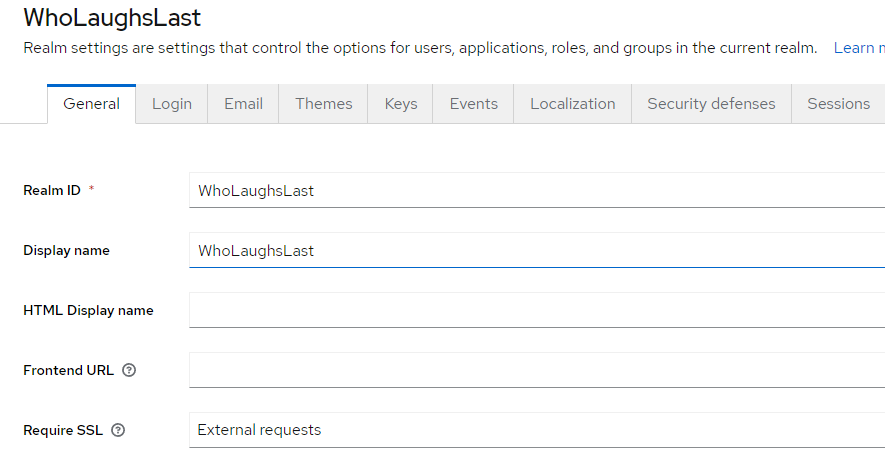
\includegraphics[scale=0.5]{keycloak-login}
	\label{keycloak-login}
\end{figure}

\subsubsection{Többjátékos mód megvalósítása}
Mivel a társasjáték csak akkor tud működni ha legalább ketten játszanak vele, így implementálnom kellett olyan funkciókat amik lehetővé teszik, hogy értesüljenek 
a felhasználók egymás lépéseiről. Mivel a kliens alkalmazás minden felhasználó gépén külön fut, így természetes, hogy a backenden kell ezt a funkciót megvalósítani, hiszen ez az egyetlen közös pont a játékosoknál. Ennek a funkciónak a megvalósításához kétféle ötlet létezik. A Server-Sent-Events (SSE) vagy a Websocket. Mindkettő olyan technológiák, amelyek lehetővé teszik a kliens és a szerver közötti valós idejű kommunikációt a weben keresztül, de különböznek a működésük és a használatuk szempontjából.

Websocket esetében kétirányú kommunikációt tesz lehetővé, ami azt jelenti, hogy mind a kliens, mind a szerver küldhet üzeneteket egymásnak bármikor. A kapcsolat felépítéséhez WebSocket protokollt használja, ami később egy WebSocket kapcsolathoz vezet.
 
Az SSE esetében egyirányú kommunikációt biztosít a szerverről a kliens felé. Csak a szerver küldhet adatokat a kliensnek. Az SSE beépített támogatást nyújt az automatikus újraépítéshez, ami azt jelenti, hogy ha a kapcsolat megszakad, a böngésző automatikusan megpróbálja újraépíteni. Könnyen használható és könnyen implementálható a böngészőben, és a szerveroldalon is könnyen konfigurálható. Mivel az én esetemben csak a klienst kellett értesíteni, hogy a játék állása, státusza megváltozott így a SSE technológiát választottam (\ref{sse}.ábra). 
\begin{figure}
	\caption{SSE szerver osztály annotációi}
	\centering
	\begin{lstlisting}[language=java,breaklines=true]
		
@RestController
@CrossOrigin(origins = "http://localhost:3000")
@Component
public class EventSender {
		
	public List<SseEmitter> emmitters = new CopyOnWriteArrayList<SseEmitter>();
		
	\end{lstlisting}
	\label{sse}
\end{figure} 
\subsubsection{Tesztelés}
A backendAPI teszteléséhez, frontend nélkül, kiváló megoldást kínál a Postman\cite{postman}, így ezt használtam a fejlesztés során. Az alábbiakban néhány kulcsfontosságú jellemzőt és funkciót ismertetek, amit a Postman kínál:

\begin{itemize}
	\item \textbf{API Tesztelés:} Egyszerűen küldhetünk http-kérést amit a sokféleképpen konfigurálhatunk. Például a fejlécben megadhatunk új kulcs-érték párokat, a kérés törzsében adhatunk meg adatokat, ennek a formátumát is beállíthatjuk. A választ is kijelzi a rendszer,így tudjuk, hogy milyen értékkel tér vissza a végpontunk, vagy esetleg valami hibára futott a kérés. 
	\item \textbf{Környezetek és változók:} Lehetőségünk van környezeteket és változókat definiálni a kérésekben, ami lehetővé teszi különböző környezetek (pl. fejlesztési, tesztelési, élő) közötti könnyű váltást és paraméterezést.
	\item \textbf{Automatizálás:} Automatizálhatjuk az API-teszteket és kéréseket. Például létrehozhatunk kollekciókat, amelyeket később futtatni tudunk, így egyszerre akár az összes végpontunkat le tudjuk tesztelni. 
	\item \textbf{Hitelesítés és biztonság:} A Postman lehetővé teszi különböző hitelesítési mechanizmusok, például API kulcsok vagy OAuth használatát. Ennek a funkciónak nagy hasznát vettem, mivel a hitelesítést megkövetelő végpontokat így tudtam tesztelni. 
\end{itemize}




\newpage



\section{Önálló munka bemutatása}
Első részben az alkalmazás backendjét írtam meg, mert felépítésben így tűnt
logikusnak. Az osztályokat rétegekbe rendeztem funkciójuk és függőségeik szerint.
\subsection{Backend}
\subsubsection{Controller és logika}
A backend részét a Java Spring projektben valósítottam meg. Ehhez a Spring Initializr-t használtam, mivel meggyorsítja a projekt létrehozásának a feladatát. Itt
egyszerűen meg lehet adni, hogy milyen függőségeket szeretnénk használni a projektünk során, majd ezután egy zip fájlként le is tölthetjük a gépünkre. Ebben a projektben bekerülnek azok az xml tag-ek a pom.xml fájlba, amik leírják a függőségeinket. Ehhez természetesen a fejlesztés során is rakhatunk hozzá újabb függőségeket
A Model rétegbe tettem azokat az osztályokat, amiket majd, később a hálózaton elküldök egy
http (HyperText Transfer Protocol) kérésbe ágyazva a szervernek, majd a válaszokat is ezekbe
az osztályokba konvertálom át. Az egész backenden ezekkel az objektumokkal dolgozok.
A DAL (Data Acces Layer)-be tettem azokat az osztályokat amik kommunikálnak a
szerverrel. Esetünkben a nevezéktan egy kicsit megtévesztő, hiszen hagyományos web
alkalmazás esetén ez a réteg az adatbázissal kommunikál, ám ennek hiányában nekünk erre
nincs lehetőségünk. Az elnevezést viszont megtartottam, hiszen gondolhatunk a szerverünkre,
mint egy okos adatbázisra, ami ismeri a ki nevet a végén társas szabályait, valamint, ha egy
másik fejlesztő olvasná a kódomat, egyből tudná, hogy az adott rétegnek mi a felelőssége.
Ezekben az osztályokban indítom el a http kéréseket, valamint a válaszokat is itt konvertálom
vissza DTO (Data Transfer Object)-re és adom tovább a BLL (Buisness Logic Layer)
rétegnek.
A BLL rétegnek különösebb jelentősége nincs. Megvalósítottam viszont, hiszen sosem lehet
tudni, hogy mikor kell továbbfejleszteni, egy új funkcióval bővíteni az alkalmazást, aminek a
logikájának a megírását ebben a rétegben kell implementálni. Hagyományos esetben itt
végeznénk el az adatok esetleges transzformációját, az üzleti logikánk itt valósulna meg. Az
én esetemben viszont erre nincsen szükség hiszen már a konzisztens adatot (vagy esetleges
hibaüzenetet) kapom vissza, közvetetten a szervertől, így itt csak egy továbbhívás történik a
DAL réteg felé. Ha esetleg API verzióváltás történne a szerveren, itt lehetne véghezvinni az adatok esetleges konverzióját az új formátumra.
A Controller rétegben definiálom azokat az API végpontokat, amiket majd a később megírt
frontendem fog hívni. Ez a réteg indítja el a kérések sorozatát, ami végigfut a backenden,
majd visszatér a szervertől kapott adattal (\ref{backend-pipeline}. ábra).

Ahogy már korábban említettem, a munkahely által biztosított szerverre kellett http kéréseket
küldeni. Ehhez volt egy Swagger\cite{swagger} oldal, hogy milyen API végpontok vannak a szerveren, és
azokhoz milyen URL tartozik.  Az is le volt írva, hogy milyen DTO-kat kell definiálni a
kommunikációhoz. Ezért így először létrehoztam a DTO, avagy Model mappát, ahol deklaráltam a
megfelelő osztályokat. A dokumentációban részletezve volt, hogy bizonyos híváshoz milyen
paramétert kell átadni, valamint mit fog visszaadni. Például, ha egy új táblát szeretnék
felvenni, akkor az adott POST kérésnél milyen DTO-t kell elküldeni, és milyen objektumot
fog visszaküldeni. Ez általában a http kérés body-jában küldték, onnan kellett kikonvertálni. Szerencsére ez Spring keretrendszernek hála, nagyon könnyen meg tudtam csinálni (\ref{post-vegpont}.ábra).
\begin{figure}
	\caption{Egy post végpont a backenden}
	

	\begin{minipage}{\textwidth}
	\begin{lstlisting}[language=java,breaklines=true]
		
@PostMapping("/board")
public ResponseEntity<?> createBoard(@RequestBody CreateBoardDTO board) {
	BoardDTO createdBoard = null;
	try {
		createdBoard= boardService.createBoard(board);
		
	}catch (ErrorCodeException e) {
		return new ResponseEntity<>(e.getErrorCode().
		getErrorCode(),HttpStatusCode.valueOf(400));
	}
	catch(Exception e){
		System.out.println(e);
	}
	return new ResponseEntity<>(createdBoard,HttpStatusCode
	.valueOf(200));
}
	\end{lstlisting}
\end{minipage}

	\label{post-vegpont}
\end{figure} 

Magán a szerveren a játék logikája már implementálva volt, így mindig
konzisztens adatokat kaptunk vissza, tehát például egy táblán nem lehet két ugyanolyan nevű
játékos. Ha esetleg egy ilyen kérés érkezett akkor egy ErrorMessage osztállyal tért vissza,
amiben részletezve volt a hiba.

\begin{figure}
	\caption{Egy kérés kiszolgálásának folyamata}
	\raggedleft 
	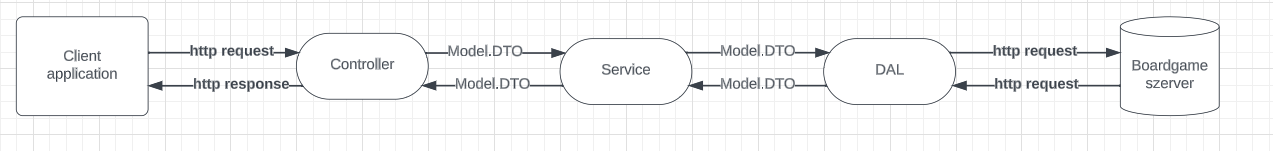
\includegraphics[scale=0.45]{backend-pipeline}
	\label{backend-pipeline}
\end{figure}

\subsubsection{Tesztelés}
Az implementáció után a kód tesztelése volt hátra, mivel az iparban elvárt a tesztesetek írása hiszen számos előnnyel jár.
Egységtesztelést végeztem, ami azt jelenti, hogy mindig csak egy alap funkciót teszteltem le, ez általában egy osztály és annak függvényei. Többféle tesztelés is létezik, például integration test, ami az egységek együttműködését teszteli, valamint end-to-end tesztek amik az egész alkalmazást fedik le. Az a jó hogyha lefelé haladva ezen a tesztelési hierarchián, egyre több tesztünk van. Egységtesztelés 
alatt a fejlesztők sok mindenre rájöhetnek a kódbázissal kapcsolatban. Például hogy a felelősségeik hogyan vannak elosztva. Ha egy osztályt nehéz tesztelni, az valószínűleg azért van, mert nagyban függ más komponensektől. Ez egy jele annak, hogy rossz a design a kódban, hiszen hogyha egy osztály nagyban függ más osztályoktól, akkor ha azok megváltoznak, az erre is hatással lesz így a fenntarthatóság jóval nehezebb lesz. A tervezésnél fontos, hogy lazán csatoltak legyenek az osztályok, hogy ilyen ne fordulhasson elő. Másik fontos előnye a tesztek írásának, hogy amikor újraírunk egy kódrészletet, esetleg gyorsabbá, vagy jobban olvashatóvá akarjuk tenni, akkor a tesztek segítségével ellenőrizhetjük, hogy megmaradt-e a kívánt funkcionalitás.  Mivel rétegeltem, a különböző funkciókat így könnyedén tudtam tesztelni őket, hiszen
egy mockolás (a Mockito [7] könyvtárat használtam ehhez) után egyszerűen tudtam tesztelni (\ref{mocking}.ábra).
A "mockolás" egy olyan technika, amelyben a tesztelés során a valódi rendszerek vagy
komponensek helyett szimulált, viselkedést utánzó objektumokat (mock objektumokat) használnak.
A mock objektumok olyan mesterségesen létrehozott objektumok, amelyek az
eredeti rendszer vagy komponens egy részét helyettesítik, és előre definiált válaszokat adnak a
függvényhívásokra vagy metódusokra. A mock objektumok segítségével szimulálhatók a
valós környezetben előforduló esetek, például adatbázishoz való kapcsolódás vagy hálózati
kommunikáció, anélkül, hogy a valódi rendszerre vagy szolgáltatásra támaszkodnánk. Ez a terv jó design esetén is szükséges hiszen, nem lehet teljesen független modulokból egy működő alkalmazást csinálni, valamiféle együttműködés feltétlen szükséges. 
\begin{figure}
	\caption{Függőségek mockolása a tesztben}
	\raggedleft
	\begin{lstlisting}[language=java,breaklines=true]
		
public class GamePlayDAOTest {
		
	GamePlayDAO gamePlayDAO;
		
	HttpClientFactory httpClientFactory;
		
	HttpClient client;
	HttpResponse response;
	
	@BeforeEach
	void mocking () throws Exception{
		httpClientFactory = mock(HttpClientFactory.class);
		client = mock(HttpClient.class);
		response = mock(HttpResponse.class);
		gamePlayDAO = new GamePlayDAO(httpClientFactory);
		when(httpClientFactory.getNewHttpClient())
		.thenReturn(client);
		when(client.send(any(),any())).thenReturn(response);
	}
	\end{lstlisting}
	\label{mocking}
\end{figure} 
\subsubsection{Többjátékos mód}
Ahhoz hogy többjátékos módot támogassa a backend, a Server-Sent-Events technológiát alkalmaztam és implementáltam le. Itt a munkahelyi szerveren létre volt hozva egy interfész,WhoLaughslastMessagingProcessor néven, amit implementálni kellett (\ref{messproc}.ábra). Alapvetően 4 darab eseményről értesítjük az összes felhasználót: \begin{enumerate}
	\item Felhasználó dobott a kockával.
	\item Felhasználó lépett egy bábuval.
	\item Játékos csatlakozott egy táblához.
	\item A játék státusza megváltozott (Például egy játékot elindítottak akkor CREATED státuszról STARTED állapotba kerül).
\end{enumerate}
Az első esetben az adat amit küldünk a kliens alkalmazásnak az új pálya helyzetét leíró adatok. Tehát hogyha egy játékos lépett akkor a bábu helyzete, a visszaküldött JSON válaszban már az újat reprezentálja. A második esetben megkapjuk, hogy hányast dobott az adott játékos, valamint ki a soron következő játékos. A 3. és a 4. esetben az új táblát leíró JSON adatot küldi el. Azok az osztályok amiket itt elküld, azok a munkahelyi szerverről származnak, ott hívják meg őket a megfelelő objektumokkal. Viszont mivel a frontendről kialakítottuk a kapcsolatot, ezeket az eseményeket mind megkapja az alkalmazás. Viszont ilyen esetben egy olyan probléma merül fel, mivel egyszerre akár többen is használhatják az alkalmazást, tehát nem biztos, hogy csak 1 tábla van használatban akár lehet több is. Hiszen tegyük fel, hogy egyszerre 2 társaság dönt úgy, hogy játszik az alkalmazással, akkor azokat az eseményeket amik az ő táblájukon történik, másik társaság kliens alkalmazása is megkap. Ez természetesen megengedhetetlen, hiszen ha az egyik társaság befejezi a játékot és a táblájuk a FINISHED státuszra vált, akkor a másik társaság játéka is befejeződne, akár kész vannak, akár nem. Tehát meg kell valahogy különböztetni a küldött eseményeket, mégpedig táblánként, hogy az adott eseményekre való feliratkozásnál csak azokra figyeljen, ami a releváns pályán történik. Eseményt az \textit{EventSender} osztály \textit{send} metódusával lehetséges. Itt megadhatunk paraméterben egy szöveget, ami az eseménynek a neve lesz, amire később referálhatunk a frontenden, hogy melyik eseményre akarunk hivatkozni. Itt paraméterben adtam meg a táblának az \textit{id} tulajdonságát, ami minden táblánál egyedi. Így biztosítani tudtam, hogy a feliratkozásnál, csak a releváns táblára iratkozik fel, így nem lesz probléma egyidejű játéknál több felhasználónál. 
\begin{figure}
	\caption{WhoLaughslastMessagingProcessor interfész implementálása}
	\begin{lstlisting}[language=java,breaklines=true]	
@Component
@RequiredArgsConstructor(onConstructor = @__(@Autowired))
public class MessagingProcessor implements WhoLaughLastMessagingProcessor{
	private final EventSender sender;
	@Override
	public void playerUpdated(PlayerUpdateMessage playerUpdateMessage) {
		System.out.println("PlayerChange"+playerUpdateMessage
		.getBoardId());\begin{environment-name}
			content
		\end{environment-name}
		sender.sendEvents("PlayerChange"+playerUpdateMessage
		.getBoardId(),playerUpdateMessage);
	}
	@Override
	public void rolledDice(RolledDiceMessage rolledDiceMessage) {
		sender.sendEvents("RollChange"+rolledDiceMessage
		.getBoardId(),rolledDiceMessage);
	}
	@Override
	public void move(PositionsUpdateMessage positionsUpdateMessage) {
		
		sender.sendEvents("PositionChange"+positionsUpdateMessage
		.getBoardId(),positionsUpdateMessage);
	}
	@Override
	public void gameStatusChange(BoardStatusChangeMessage
		boardStatusChangeMessage) {
		sender.sendEvents("StatusChange"+boardStatusChangeMessage
		.getBoardId(),boardStatusChangeMessage);
	}
}
		\end{lstlisting}
		\label{messproc}
	\end{figure} 
	\FloatBarrier
Valamint még szükség volt arra az osztályra (\ref{eventsender}.ábra) ami magát az eseményeket elküldi a kliens számára.  Egy \textit{SseEmitter} osztályú objektumokból álló listát is létrehoztam mint tagváltozó, itt tárolom a különböző klienseknek a feliratkozását. Ez nagyon fontos, hogy CopyOnWriteArrayList típusú legyen, mivel így kezelhető a konkurencia.Valamint létrehoztam egy újabb végpontot, amit majd az \textit{EventSource} létrehozásánál hivatkozhat a frontend.  Ha ez a hívás megtörténik, akkor először létrehozok egy emittert, aminek konstruktorában a \textit{\texttt{LONG.MAX\_VALUE}} értéket adom. Ez az érték azt jelenti, hogy egyes emitterek mennyi ideig tartsák fent a kapcsolatot mielőtt megszakítják a kapcsolatot. Ezek után létrehozok egy \textit{SseEmitter} osztályú objektumot ami küld egy \textbf{"INIT"} nevű eseményt, majd ezt az emittert az osztály tagváltozójához hozzáadom. Deklaráltam egy függvényt \textit{sendEvents} néven, ami végigiterál ezeken az emitter-eken, és elküldi a paraméterben átadott névvel és adattal, az eseményt a kliens alkalmazásnak.   
\begin{figure}[ht]
	\caption{EventSender osztály implementálása}
	\begin{minipage}{\textwidth}
	\begin{lstlisting}[language=java,breaklines=true]	
@RestController
@CrossOrigin(origins = "http://localhost:3000")
@Component
public class EventSender {
		
	public List<SseEmitter> emmitters = new CopyOnWriteArrayList
	<SseEmitter>();
		
	@RequestMapping("/subscribe")
	public SseEmitter subscribe() {
	System.out.println("Subscripbed");
		SseEmitter emmitter = new SseEmitter(Long.MAX_VALUE);
		try{
			emmitter.send(SseEmitter.event().name("INIT"));
		}catch (IOException e) {
			e.printStackTrace();
		}
		emmitter.onCompletion(() -> emmitters.remove(emmitter));
		emmitters.add(emmitter);
		return emmitter;
		
	}
	public void sendEvents(String eventname, Object data){
		for(SseEmitter emitter : emmitters){
			try{
				emitter.send(SseEmitter.event().name(eventname)
				.data(data));
			}catch(IOException e){
				emmitters.remove(emitter);
			}
			}
		}
	}
	\end{lstlisting}
	\end{minipage}
	\label{eventsender}
\end{figure} 
\FloatBarrier


\subsection{Autentikáció}
\subsubsection{Backend}
Az autentikációt a Keycloak nyílt forráskódú keretrendszerrel valósítottam meg. Ehhez, hogy konfigurálni tudjam a 
szükséges beállításokat, és futtatni tudjam otthoni környezetben, legegyszerűbb megoldásnak tartottam, hogy egy Docker konténerben 
futtattam. Ehhez először telepíteni kellett a Dockert, majd a terminálban kiadni a következő parancsot: 
\textbf{docker run -p 10000:8080 -e KEYCLOAK\_ADMIN=admin -e KEYCLOAK\_ADMIN\_PASSWORD=\\admin quay.io/keycloak/keycloak:22.0.5 start-dev}
Itt lehetett beállítani, hogy a keycloak melyik porton fusson. Mivel a backendem spring boot alkalmazás aminek az alapértelmezett portja 8080 így 
ettől eltérően kellett választani, ami a 10000 lett. A parancs segítségével letöltöttem a megfelelő Docker Imaget amit már könnyedén el lehetett indítani,
és elérhetővé vált számomra a \textbf{localhost:10000} -en keretrendszer. Az admin konzolba való belépés után lehetett beállítani a kívánt funkciókat. 
Először is egy új realm-et hoztam létre aminek a neve: WhoLaughsLast. A realmeken belül lehet létrehozni a clients listát amik esetünkben az alkalmazásokat jelentik (\ref{keycloak}.ábra). Így létre is hoztam egyet: \text{who\_laughs\_last\_client} néven majd ehhez a client-hez rendeltem hozzá a felhasználókat. 
Pár beállítást még kellett végezni a client-en. Először is megadtam a egy érvényes átirányítási URL-t. Ez azt az elérési utat adja meg, ahova bejelentkezés után navigálni akarunk. Én 
a \textbf{http://localhost:3000/*} adtam meg, hiszen ezen a porton futott nekem a frontend alkalmazás, így a felhasználó bejelentkezés után bent volt az alkalmazásban. A keycloak
széles API-t kínál így ezt megismerve az backendemről autentikáció során ide küldtem a kéréseket. Azt is be lehet állítani, hogy a mennyi idő után jár le az access token érvényessége, tehát utána majd újat kell kérni a szervertől. 
\begin{figure}
	\caption{Keycloakban a clients lista részlete}
	\centering
	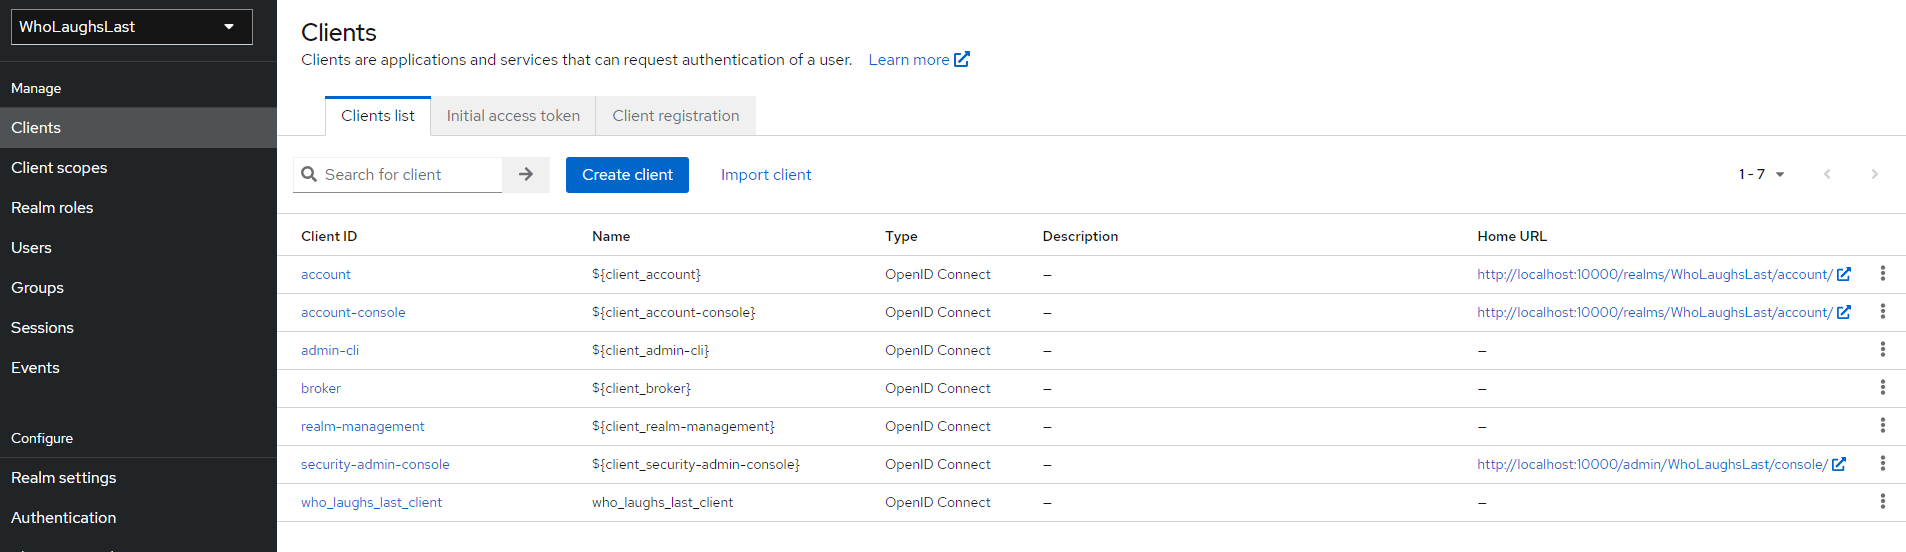
\includegraphics[scale=0.5]{keycloak-cients}
	\label{keycloak}
\end{figure}
\FloatBarrier


A végpontok biztonságossá tételéhez a \textbf{Spring Security}-t és az \\ \textbf{OAuth2ResourceServer} dependency-ket használtam fel. A függőségeket leíró xml-eket beillesztettem a pom.xml fájlba, majd a Maven letöltötte őket, hogy majd használni tudjam (\ref{pom}.ábra).
\begin{figure}
	\caption{A pom.xml fileban a függőségek}
	\centering
	\begin{lstlisting}[language=XML,breaklines=true]
<dependency>
	<groupId>org.springframework.boot</groupId>
	<artifactId>spring-boot-starter-oauth2-resource-server</artifactId>
	<version>3.1.5</version>
</dependency>
<dependency>
	<groupId>org.springframework.boot</groupId>
	<artifactId>spring-boot-starter-security</artifactId>
	<version>3.1.5</version>
</dependency>
	\end{lstlisting}
	\label{pom}
\end{figure}
\FloatBarrier


Miután a Spring Security bekerül az alkalmazásba, alapértelmezetten csinál egy SecurityFilterChain-t ami megköveteli, hogy az összes API végpontnál
a hívónak autetntikálnia kell magát. Ezt a függvényt kell felülírni és úgy implementálni ahogyan azt mi szeretnénk. \textbf{@Bean} annotációval van ellátva,
így ezt a Spring kezeli és tudja, hogy mikor kell használni. Amikor a kérések beérkeznek az alkalmazásunkba, akkor végighaladnak ezeken a szűrőkön amiket beállítunk. Miután talál 
egy olyan filtert ami a kéréshez illik: Például a "/board" végződésű végpontra jött kérés, akkor azt tudja, hogy autentikálni kell, és a többi filtert már nem nézi meg, akár illik rá akár nem. 

\begin{figure}
	\caption{SecurityFilterChain működése }
	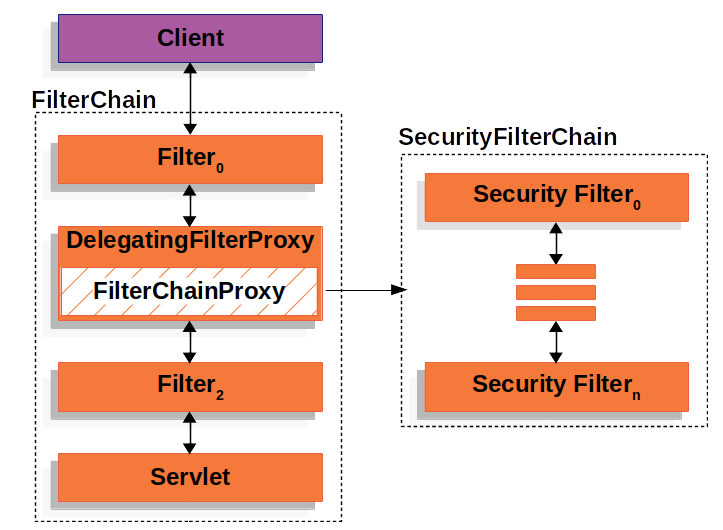
\includegraphics[scale=0.45]{filterchain}
\end{figure}


Úgy konfiguráltam fel a függvényt, hogy 3 végponton kívül mindent authetnikáljon: \textbf{/auth/createToken}, \textbf{/auth/refreshToken} ,\textbf{/subscribe}. Első kettőt végpontot azért nem kell autentikálni, mivel ide érkeznek azok a kérések amikor a felhasználó be akar jelentkezni, és kapja meg a szükséges token-eket amikre majd később szüksége lesz az autentikációnál. Ezek után a OAuth2 resource szervert kellett felkonfigurálni. Az application.yml file-ban írtam bele a különböző elérési utakat amikre a szervernek szüksége van, hogy autentikálni tudja a jwt \footnote{Json Web Token} tokeneket. A keycloak-nál a \textbf{http://localhost:10000/realms/WhoLaughsLast\\/protocol/openid-connect/certs} elérési úton 
elérhető az adott client-hez tartozó autetnikációs adatok. A jwt tokeneket a http kérések fejlécében küldtem el mint BearerTokenek. Hogy ezekhez hozzá tudjak jutni,
egy Convertert kellett írni, majd a OAuth szerver ellenőrizze a hitelességüket. 

\begin{figure}
	\caption{SecurityConfig implementálása}
	\centering
\begin{lstlisting}[language=java,breaklines=true]
@Bean
public SecurityFilterChain securityFilterChain (HttpSecurity http) throws Exception{
	http
	.cors().and()
	.csrf()
	.disable()
	.authorizeHttpRequests(authorize -> authorize.
	requestMatchers("/auth/createToken","/subscribe","/auth/refreshToken")
	.permitAll()
	.anyRequest().
	authenticated()).oauth2ResourceServer()
	.jwt().jwtAuthenticationConverter(jwtAuthConverter);
	http
	.sessionManagement()
	.sessionCreationPolicy(STATELESS);
	
	return http.build();
}
\end{lstlisting}
\label{secConf}
\end{figure}
\FloatBarrier


Ezek után implementáltam az autentikációs végpontot (\ref{authEndpoint}. ábra). Létrehoztam egy új Controllert aminek AuthController lett a neve,
hogy elkülönítve legyen a többi végponttól ami a játékhoz kell, az átláthatóság és a rendezettség érdekében. Az egyik végpont 
funkciója az, hogy egy paraméterben kapott authorization code-ot elküldi a keycloak végpontjára amiért cserébe egy refresh tokent és egy access tokent kap,
és ezeket juttatja el a frontendre. A másik végpont funkciója pedig az, hogy egy paraméterben kapott refresh tokent beváltva új access tokent kapjon a frontend az autentikációhoz. 

\begin{figure}
	\caption{Autentikációs végpont}
	\centering
	\begin{lstlisting}[language=java,breaklines=true]
		
@PostMapping("/createToken")
public TokenDTO createToken(@RequestBody AuthTokenDTO authCode) throws Exception{
	return authService.getTokens(authCode.getAuthCode());
}		

@PostMapping("/refreshToken")
public TokenDTO refreshAccesToken(@RequestBody RefreshTokenDTO refreshTokenDTO)
throws Exception{
	return authService.refreshAccesTokenWithRefreshToken(refreshTokenDTO
	.getRefresh_token());
}
		
	\end{lstlisting}
	\label{authEndpoint}
\end{figure} 

\begin{figure}
	\caption{Postman autentikációs token kérés}
	\label{fig:postman}
	\centering
	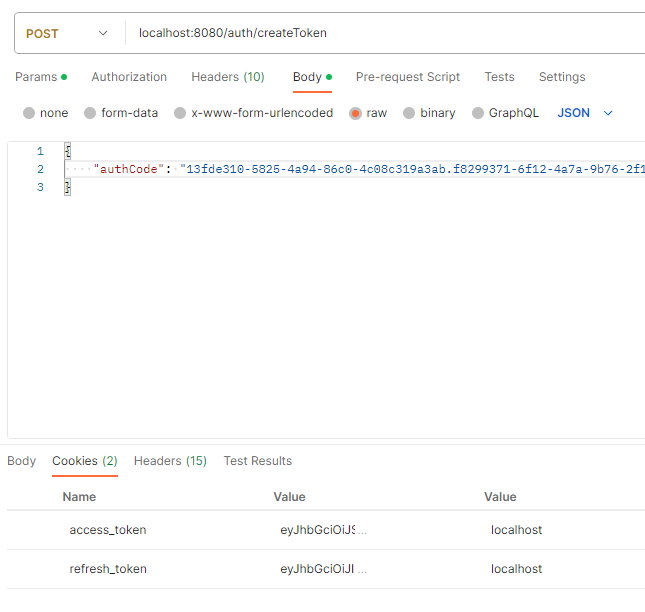
\includegraphics[scale=0.5]{getTokens}
\end{figure}

\subsubsection{Frontend}
A frontenden az autentikáció egyik feladata az authorization code eljuttatása a backend-re volt. Mivel használni akartam a keycloak által 
készített login paget, így az URL-ből kellett kivennem a code-nak az értékét. Mivel a megfelelő bejelentkezés után a keycloak átnavigál a frontend 
URL-jére, hiszen ezt beállítottuk az admin oldalon, így ezt az eseményt fel tudtam használni. Vue Routert használok a navigációra az alkalmazáson belül. A Vue Router 
sok hasznos funkcióval rendelkezik, de ennél a problémánál a navigációs őröket (Navigation Guards) tudtam felhasználni. Itt meg tudok adni egy függvényt ami
mindig meghívódik azelőtt, hogy navigáció történne az alkalmazáson belül. Tehát amikor megtörténik a navigáció a keycloak-os felületről az alkalmazásra, a függvény amit 
definiálok le fog futni. Paraméterként megkapom azt az elérési utat ahonnan navigáltak, valamint azt is ahonnan navigáltak. Mivel ahonnan navigálunk el ott jelenik meg az
authorization code, így ki tudom nyerni onnan (\ref{authCode}.ábra). Egy újabb Pinia Store-t is definiáltam az autentikációhoz köthető függvények miatt a jó strukturáltság érdekében. Definiáltam egy \textbf{authTokens} változót is ami az éppen aktuális access és refresh tokeneket tartalmazza. Itt implementáltam egy API hívást, ami http kérés törzsében tárolja az authorization code-ot és küldi el a backend számára. A választ eltárolom az authTokens változóban, így ezekkel már el tudom érni a backenden a játékhoz tartozó védett végpontokat is. 
\begin{figure}
	\caption{Authorization code kinyerése az elnavigált URL-ből}

		\begin{minipage}{\textwidth}
			\begin{lstlisting}[style=javascriptStyle]
				router.beforeEach(async (to,from,next) => {
					const authStore = useAuthenticationStore();
					if(to.query.code) {
						await authStore.getAuthTokens({code: to.query.code});
						next(to.path);
					}
					else if(to.name === "playing" && !from.name) {
						next("/boardManagement");
					}
					else {
						next();
					}
					
					
				})
			\end{lstlisting}
		\end{minipage}
	
	\label{authCode}
\end{figure}
\FloatBarrier

A másik fontos dolog volt implementálni az új access token kérését frontenden. Amint lejárt az addig használt access token érvényessége a szerver 401-es Unauthorized 
hibakóddal tért vissza. Ilyenkor kellett a refresh tokent használni, hogy új access tokent kapjunk. Az axios könyvtárat használtam a http kérések küldésére. Az axios 
használatakor létrehozunk egy példányt belőle amik tartalmazzák azokat a függvényeket amikkel a http kéréseket el tudjuk küldeni, például a GET,POST,DELETE,stb\ldots Amikor létrehozunk egy ilyen példányt, konfigurálhatjuk úgy, hogy minden egyes kérés küldésekor vagy válasz fogadásánál, bizonyos dolgokat végezzen el. Nekem arra volt szükségem, hogy minden kérés elküldésekor a http fejlécébe csatolja az éppen aktuális access tokent, hogy majd a backend autentikálni tudja. Valamint minden egyes beérkezett válasznál ellenőriznem kellett, hogy a válasz 401-es hibakóddal tér-e vissza, mert akkor lejárt az access token, és újat kell kérni. Így ebben a részben hívtam meg az implementált API kérést, majd az újonnan kapott tokent eltároltam a Store-ban, majd ezek után újra elküldtem a meghiúsult API kérést. Mivel egy 
pinia store-ban tároltam el az autentikációs tokeneket, így ha a felhasználó frissíti az oldalt, ezek mind elvesznek. Így erre az eshetőségre is fel kellett konfigurálni az API hívásokat, hogyha nincsenek tokenek, akkor navigáljon el a bejelentkező oldalra. Ilyenkor viszont azt az API hívás amit a frissítés után akarunk végre-hajtani, eldobjuk. Viszont ez nem jelenti azt, hogy minden egyes frissítéskor be kell jelentkeznünk, hiszen a Keycloak számon tartja, hogy be vagyunk jelentkezve, ezért rögtön vissza is navigál arra az URL-re amit megadtunk neki (\ref{axiosConfig}.ábra).

\begin{figure}
 	\caption{Axios hívások felkonfigurálása autentikáció kezelésére}
 	
 		\begin{minipage}{\textwidth}
 			\begin{lstlisting}[style=javascriptStyle]
 				const AxiosWithToken = axios.create({
 					baseURL: 'http://localhost:8080/'
 				});
 				
 				AxiosWithToken.interceptors.request.use(config => {
 					const authStore = useAuthenticationStore();
 					if(authStore.authTokens){
 						config.headers.Authorization = `Bearer ${authStore.authTokens.access_token}`;
 						return config;
 					}
 					
 				})
 				
 				AxiosWithToken.interceptors.response.use(response =>{
 					return response;
 				},async error=> {
 					const authStore = useAuthenticationStore();
 					if(error.response.status === 401 && authStore.authTokens.refresh_token) {
 						await authStore.getNewAccesTokenWithRefreshToken();
 						return AxiosWithToken(error.config);
 					}
 					else if(!authStore.authTokens.access_token){
 						window.location.href="http://localhost:10000/realms/WhoLaughsLast/protocol/openid-connect/auth?response_type=code&client_id=who_laughs_last_client";
 						return Promise.reject(error.config);
 					}
 				})
 			\end{lstlisting}
 		\end{minipage}
 	
 	\label{axiosConfig}
\end{figure}
\FloatBarrier

\newpage

\subsection{Frontend}
\subsubsection{Komponensek és játékmenet}
A frontend készítésnél már volt egy kiinduló gitlab projektem, amit a külső konzulensem
biztosított számomra. A gitlab egy olyan szoftver amit rendkívül gyakran használnak a szoftverfejlesztésben. A lényege, hogyha közösen többen fejlesztenek egy alkalmazást, akkor a különböző kódrészleteket egy helyre töltik fel a fejlesztők, és így áll össze az alkalmazás. Éppen az aktuális verziót le tudják tölteni a saját gépükre, így látják a változtatásokat amiket végbementek. Ez a projekt egy üres projekt volt, de a Vue.js keretrendszer, webpack
konfiguráció már importálva volt, valamint sok hasznos könyvtárat tartalmazott. Ahogy
korábban említettem, a Vue.js egy komponens orientált fejlesztés tesz lehetővé. Ezt használva
először azt terveztem meg, hogy milyen komponensekből fog állni a megjelenítés.
Először a táblák megjelenítéséért felelős komponenst írtam meg. Ez listázza az összes
szerveren lévő táblát. Itt iratkozok fel a szerver által küldött SSE eseményekre is, hiszen ez az első olyan komponens amit lerenderel a böngésző, így ennek a kódja fut le először. A Vue komponensekben definiálni lehet expliciten, hogy a komponens bizonyos életciklusaiban milyen függvényeket hívjon meg. Több ilyen életciklus van, például beforeMount,beforeCreated,mounted és még sok más. Én az mounted (\ref{onMounted}.ábra) életciklust definiáltam expliciten. Ilyenkor már a komponens megjelenítette a kinézetet, és működésre kész. Ha ez kész akkor kérem le a szerverről a táblákat tartalmazó adatokat és építem ki a kapcsolatot az SSE emitterel. Ebben a komponensben lehet létrehozni egy új táblát. Ez úgy történik, hogyha rákattintunk a CreateBoard gombra, akkor egy új ablak jelenik meg. Itt adhatjuk meg a táblánk paramétereit, például a nevét, hány játékossal lehet ezt játszani, hány bábuja lesz egy játékosnak, valamint, hogy két játékos kiinduló pozíciója között hány darab mező legyen. Az egyes paraméterekre bizonyos feltételek kellettek, hogy teljesüljenek, különben nem lehetett létrehozni őket a szerveren. Így egy \textit{computed} tulajdonság segítségével ellenőriztem ezeket, hogy egészen addig ne lehessen létrehozni, ameddig ezek a feltételek nem teljesülnek. Ha megadjuk a megfelelő paramétereket és rákattintunk a Create gombra, akkor elküldi a backend szervernek a kérést. Ez visszaadja nekünk a szerveren generált pályát, amihez plusz információkat csatol, például az azonosítója, valamint, hogy ki fogja kezdeni a játékot, stb\ldots Az összes szerveren lévő táblát a Pinia Storeban, egy \textit{boards} nevezetű változóban tárolom el. Mivel ez egy reaktív változó, így hogyha az értéke változik az összes, ettől függő komponens le fogja követni a változásokat. Így amikor megkapom az újonnan létrejött táblát, hozzáadom ehhez a \textit{boards} tömbhöz, így rögtön frissülni fog a felület amint a Create gombra kattintok. 

\begin{figure}
	\caption{onMounted életciklus hook meghívása a BoardManagement komponensben}
	
		\begin{minipage}{\textwidth}
			\begin{lstlisting}[style=javascriptStyle]
				onMounted(async () => {
					boardStore.eventSource = getEventSource();
					await boardStore.getBoards();
				})
			\end{lstlisting}
		\end{minipage}
	
	\label{onMounted}
\end{figure}
\FloatBarrier

Következőleg az egy táblát reprezentáló komponenst implementáltam le. Itt látszódnak a tábla
fontosabb adatai, a különböző funkciójú gombok, a Start, JoinPlayer, Reset, Stop valamint a DeleteBoard. Ezek a gombok, a DeleteBoard kivételével, függnek attól, hogy a pálya milyen állapotban van. A JoinPlayer gomb érhető csak el, hogyha még nincs meg a megfelelő számú játékos a táblához. Ha ez teljesül, akkor csak a Start gomb lesz elérhető, ami elindítja a játékot, így STARTED státuszra változik a tábla. Ezek után a Stop és a Reset gombok lesznek elérhetőkm, ahol az előbbi befejezi a játékot és FINISHED státuszba kerül a tábla, vagy az utóbbi kitörli az összes játékost a tábláról, és CREATED státuszba teszi. Ha a JoinPlayer gombra kattintunk, akkor egy feljövő ablakban tudjuk megadni a játékosunk adatait, ami a neve és a színe. Akár egy felhasználó több játékost is csatlakoztatni tud, így akár nem kell 5 különböző felhasználó ha egy 5 fős pályán akarunk játszani. Az elérhető színeket a szerverről kérdezem le, majd ezeket egy legördülő ablakban listázom ki. Itt is vannak bizonyos megkötések, minthogy a játékos neve legalább 3 karakterből kell hogy álljon, valamint nem lehet olyan színe és neve, amit már egy előbb csatlakozott játékos kiválasztott. A felületen a játékosok neveit olyan színnel jelenítem meg, amelyeket kiválasztottak. Ehhez csak egy függvényt kellett készítenem, ami megfelelő formátumra hozza a szervertől kapott színek neveit, hogy az így kapott nevet a CSS értelmezni tudja (\ref{board}.ábra). 

\begin{figure}
	\caption{Egy tábla adatainak megjelenítése}
	\label{board}
	\centering
	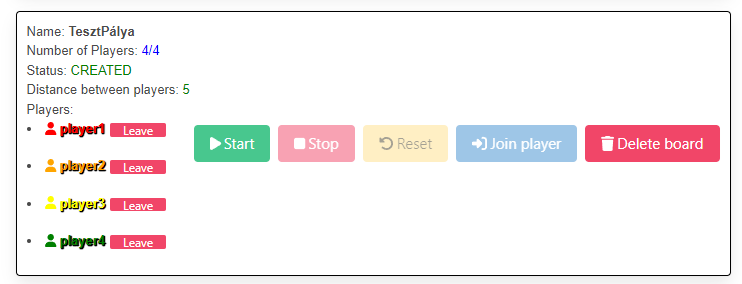
\includegraphics[scale=0.63]{board}
\end{figure}

Egy játékos megjelenítéséért, külön komponenst hoztam létre, mert így jobban el tudtam szeparálni a különböző felelősségeket a komponensek között. Egy LeavePlayer gombot is létrehoztam, hogy esetleg ha egy játékos meggondolná magát a játék kezdete előtt, ki tudjon még lépni. 
Ha egy játékos elhagyja a pályát, vagy a tábla státusza megváltozik, akkor erről a többi játékosnak is tudnia kell. Így ha egy ilyen kérés érkezik be a szerverre, az küld egy eseményt erről. Így ebben a komponensben regisztrálok fel a \textit{PlayerChange} és a \textit{StatusChange} eseményekre, hogy így majd meg tudjam jeleníteni, ha esetleg egy másik játékos elhagyta a pályát. A \textit{PlayingBoard} komponens, az ami megjeleníti a pályát és a játékosokat. A mounted életciklusában feliratkozom a \textit{RollChange} és a \textit{PositionChange} eseményekre, hiszen ez ekkor lesz releváns. 

Amint csatlakoztak a játékosok és valamelyikük elindította a játékot, átkerülünk egy új nézetbe, ami a pályát és többi játékost tartalmazza (\ref{playingboard}.ábra).
\begin{figure}
	\caption{Játék közbeni kinézet}
	\label{playingboard}
	\centering
	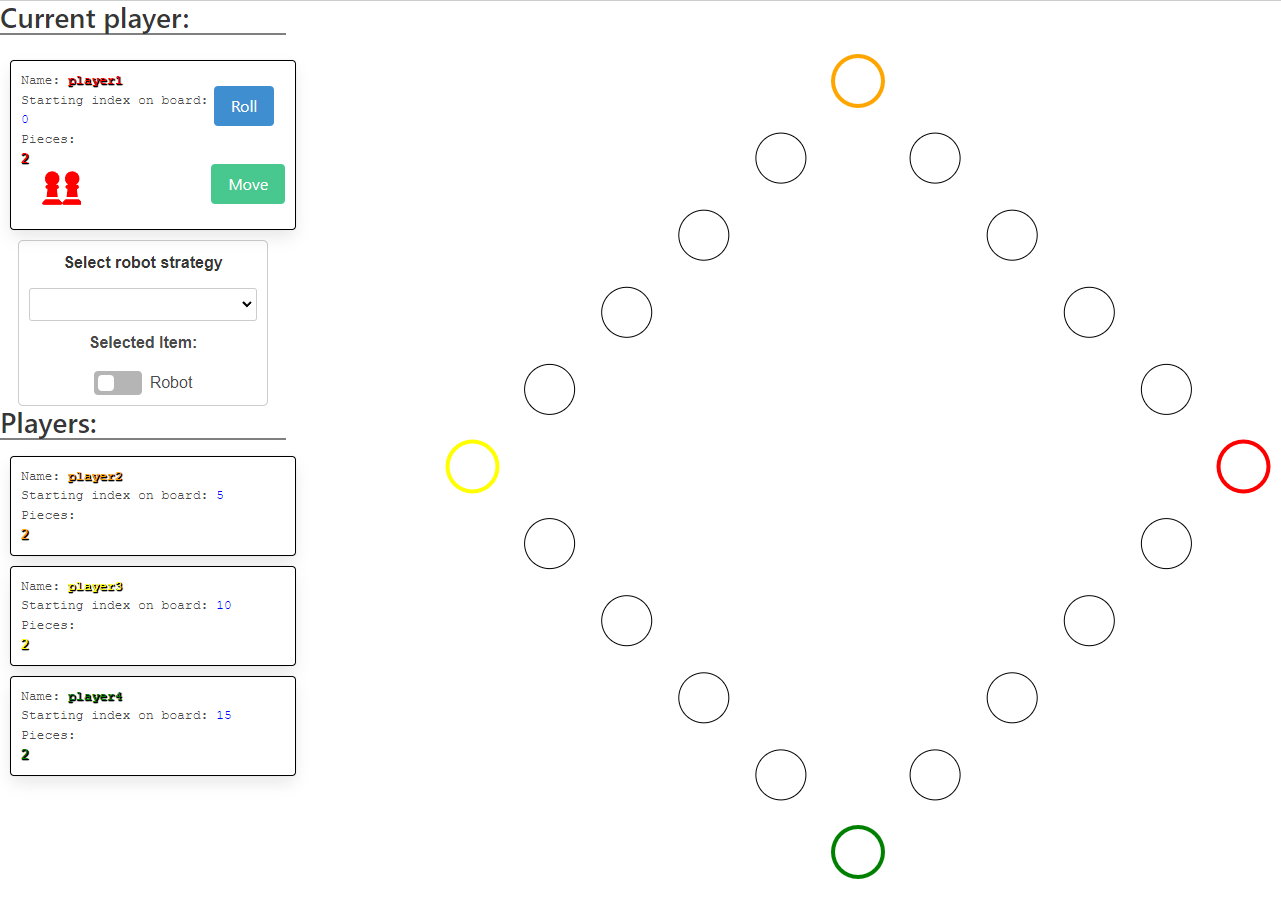
\includegraphics[scale=0.35]{playingboard}
\end{figure}
\FloatBarrier
Amikor átnavigálunk, az elindított táblát, valamint a kezdő játékost elmentem egy külön változóba, hogy később el tudjam érni. Ebben  a komponensben folyton figyeltem ezt a változót a
\textit{watch} függvénnyel, hiszen így tudtam lekövetni a változásokat amik történtek. A bal oldalon jelenítettem meg a játékosokat, az éppen soron következő játékost kicsit részletesebben. Valamint itt lehet beállítani, hogy akarjuk-e, hogy egy robot játsszon helyettünk, valamint annak a stratégiáját. A CurrentPlayer komponensben jelenítem meg, hogy a soron lévő játékosnak még hány bábuja nincs fent a táblán, valamint itt vannak a Roll és Move gombok. Először a felhasználónak a Roll gombra kell kattintania, ez szimulálja dobást. Ilyenkor egy http kérés történik a szerver felé, ami visszaad egy objektumot, a dobással kapcsolatos információkkal. Ebben benne van a dobás értéke, valamint egy token ami az adott dobáshoz tartozik. Ez a szerver által van generálva és ott van számon tartva, hogy melyik dobáshoz tartozik az adott token. Ha tudunk lépni az adott dobással, tehát vagy hatost dobtunk és ki tudunk jönni a kezdő területről, vagy már lent van bábunk a pályán, akkor meg lehet nyomni a Move gombot. Úgy implementáltam le a játék működését, hogy alapértelmezetten azt a bábut választom ki, ami a már a táblán van, ha esetleg nincs ilyen, akkor az lesz ami még nem került fel. Viszont hogy a felhasználó rákattint egy másikra, akár nem pályán lévőre, akkor avval fog mozogni. Ha nem pályán lévő bábura kattint és nem hatost dobott, akkor viszont hibaüzenetet fog kapni, hogy avval a bábuval nem lehet mozogni, hiszen onnan csak hatos dobással lehet kimenni. A \textit{watch} fügvénnyel figyelem, hogy mikor változik a soron következő játékos, és amikor változik, beállítom a választott bábut az alapértelmezettre. Ha a dobásunk hatos, akkor egy kis értesítés jelenik meg, hogy akár egy új bábut is kivihetünk a táblára.  Ha a Move gombra kattintunk, akkor előre lép annyit a bábunk amennyit dobott vagy ha még nem volt fent, akkor a kezdő pozícióra lép ki. Ehhez el kell küldeni a szervernek az adott dobáshoz tartozó tokent, amit az előző válaszban kaptunk meg, valamint a kiválasztott bábu azonosítóját. A válaszban a pálya új állapotát kapjuk meg, amit a reaktivitásnak köszönhetően rögtön meg is jelenítünk. Amint léptünk, a soron következő játékost állítjuk be, aki elvégzi az előzőekben leírt tevékenységeket. Amint valaki befejezi a játékot, rögtön egy új nézetbe visz át minden játékost az alkalmazás. Itt jelenítjük meg a játékosok állását, hogy ki hogyan szerepelt a játék alatt. A Score változó a szerver által van számolva, a bevitt bábuk száma határozza meg, így alakul ki a végeredmény (\ref{game-end}.ábra). Az Ok gombra kattintva, visszakerülünk abba a nézetbe, ahol az elérhető táblákat listázzuk ki. 

\begin{figure}
	\caption{A végeredmény megjelenítése a játék befejezése után}
	\label{game-end}
	\centering
	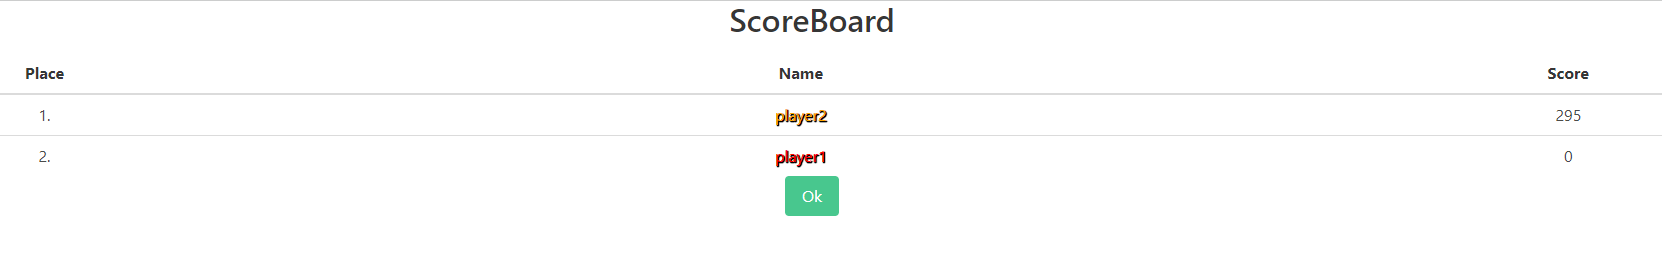
\includegraphics[scale=0.32]{game-end}
\end{figure}
\FloatBarrier
Mivel a backendem hibaüzenetet is adhat, hogyha inkonzisztens adatot küldök el, így annak
megjelenítésével is foglalkoznom kellett.Például, hogyha egy játékos dob a kockával és nem tud lépni a dobott számmal akkor, egy egyszerű piros ablak
jelenik meg az oldal tetején, amiben szerepel, hogy nem tud lépni az adott számmal.A többi hibaüzenetre is megjelenne ez az ablak, de mivel az egyes gombokat nem lehetne használni hogyha rossz adatot küldenénk a szerverre, így ez az eset nem fordul elő. Ez az ablak 2,5 másodperc elteltével eltűnik.
\subsubsection{Grafikus megjelenítés}

A játéktér megjelenítése nagyon fontos feladat volt, hiszen ez nagy mértékben befolyásolja a felhasználói élményt, így lényeges volt hogy igényes legyen. A Konva könyvtárat használtam fel ehhez ami remek eszközöket biztosít a feladat megvalósítására. 
Először a pályát kellett megrajzolnom. Amikor létrehozzuk a táblát, minden csatlakozott játékosnak van egy alap kiinduló pozíciója, ami egy szám. Ide kerülnek fel először a bábuk és ide kell visszaérkezniük. Minden bábuhoz tartozik egy \textit{positionOnTheBoard} nevű tulajdonság, ami a helyzetét adja meg a táblán. Hogyha ez -1, akkor még nem lépett ki, vagy már körbeért a pályán. A pályának a mezőit körök reprezentálják. Ilyen köröket a Konva segítségével könnyen létre tudtam hozni (\ref{konva}.ábra), és több tulajdonságot adhattam meg neki. Mivel meg akartam valósítani, hogyha rákattintunk egy mezőre, akkor az éppen azon lévő bábut válassza ki, így minden egyes körnek adtam egy azonosítót, ami azt jelzi, hogy éppen hanyadik mező a táblán. Így annyi a dolgom, hogy meg kell keresni azt a bábut, aminek a \textit{positionOnTheBoard} tulajdonsága megegyezik a kattintott kör azonosítójával, és hogyha van ilyen, akkor azt beállítani mint választott bábu .

A játéktér alakjának megrajzolása az egyik legnehezebb volt a fejlesztés során. Legelső lépés volt magának a helynek a meghatározása ahol ki fogom rajzolni a könyvtárat. Ahhoz hogy rajzolni tudjunk a felületre, létre kell hoznunk egy Stage objektumot, ami majd tartalmazza a további objektumainkat. Ennek a Stage objektum \textit{container} tulajdonságának kell beállítani azt a html elemet, ahol akarjuk hogy megjelenjen a pálya. Itt adhatjuk meg, hogy milyen széles és magas legyen (\ref{konvaStage}.ábra). 

\begin{figure}
	\caption{Konva Stage objektum beállítása}
	\begin{minipage}{\textwidth}
		\begin{lstlisting}[style=javascriptStyle]
			 const containerWidth = document.getElementById("container").offsetWidth;
			const containerHeight = document.getElementById("container").offsetHeight;
			var stage = new Konva.Stage({
				container: 'board',
				width: containerWidth,
				height: containerHeight
			});
		\end{lstlisting}
	\end{minipage}
	
	\label{konvaStage}
\end{figure}
\FloatBarrier

Mivel a játékosoknak körbe kell érniük valahogy, így a pálya elejének és végének kapcsolódnia kell egymáshoz. Ezért legegyszerűbben úgy tudtam megoldani hogyha a pálya kör alakú lesz. Viszont hogyha több mint 2 játékossal csatlakoznak a pályához, akkor elég rosszul néz ki, ha akkor is csak egy sima kör a tábla alakja. Így úgy készítettem el a kinézetét a pályának, hogyha \textit{n} játékossal csatlakoznak a pályához,és \textit{n} nagyobb mint kettő, akkor egy \textit{n}-oldalú sokszög lesz a pálya kinézete. Ennek a megvalósításához 2 függvényt írtam meg, \textit{setUpBoardWith2Player} és a \textit{setUpBoardWithMorePlayer}. Mindkét esetben paraméterben megadtam a \textit{board} objektumot, ami éppen a kirajzolandó táblának a tulajdonságait tartalmazta. A függvények elején kiszámoltam, hogy összesen mennyi mező lesz a pályán. Amikor létrehozunk egy táblát, akkor megadjuk, hogy két kezdőpozíció között hány darab mezőnek kell lennie, ez a \textit{distanceBetweenPlayers} tulajdonság. Így ki tudtam számolni, hogy \(numberOfFields = joinedPlayers * distanceBetweenPlayers\).

Először azt az algoritmust implementáltam le, amikor csak két játékos van. Itt azt akartam elérni, hogy egy kör körvonalán helyezzem el a mezőket, amik szintén kis körökből állnak. Egy kör körvonalának koordinátájának kiszámításához szükség van az adott kör sugarára, valamint a bezárt szögre. A kör sugarát megkaptam úgy,hogy a Stage objektum széllességét elosztottam kettővel. Mivel egy ciklusban rajzoltam ki köröket, ezért mindig az aktuális körnek kellett kiszámolnom  a bezárt szögét. A ciklus nullától 360-ig ment hiszen ez jelentette a teljes kört. Mivel tudtam azt is, hogy összesen hány mező lesz a táblán, így a 360-at elosztottam ezzel a számmal, és így megkaptam azt a szöget amennyivel növelnem kell az előző kör bezárt szögéhez képest. Ezt az értéket \textit{angleOffset}-nek neveztem el. Ezt az értéket még radiánba át kellett váltani mivel a \textit{Math.sin} függvény radiánban számol.  Tehát az \textit{n}-edik kör bezárt szöge: \(\alpha_{n} = \alpha_{n-1} + angleOffset\). Így az \textit{n}-edik körnek a koordinátáit ki tudtam számolni a következőképpen: 
\(x_{n} = sin(\alpha_{n})*r\),valamint \(y_{n} = cos(\alpha_{n})*r\) ahol az r a körnek a sugara. \ref{kettesPlayerKoord}.ábrán látszik, hogy még a \textit{stage.width} és a \textit{stage.height} változókat hozzáadom a koordináták értékeihez. Ez azért szükséges, hogy a kör alakú pályának a középpontja, a Stage objektumon közepén jelenjen meg. 

\begin{figure}
	\caption{Egy mező koordinátájának kiszámítása}
	\begin{minipage}{\textwidth}
		\begin{lstlisting}[style=javascriptStyle]
		 x: stage.width() / 2 + (Math.sin(angleInRadian) * boardGameradius),
	   	 y: stage.height() / 2 + (Math.cos(angleInRadian) * boardGameradius),
		\end{lstlisting}
	\end{minipage}
	
	\label{kettesPlayerKoord}
\end{figure}

Mivel a kezdő pozíciókat még valahogy szemléltetni akartam a felhasználók számára, ezért beleraktam egy feltételt, hogyha a bezárt szög osztható 180-nal, akkor a létrehozott kör körvonala olyan, színű legyen mint a játékosé. Mivel azt hogy mennyi mező legyen egy táblán a felhasználó adja meg, így ez a szám a két játékost tartalmazó táblák között is változhat. Ezért hogy egy mező éppen mekkora legyen, tehát a körnek a rádiusza függ attól, hogy a pályán mennyi mező van, így kisebb pályákon egyes mezők mérete nagyobb mint nagyobb pályákon.

Ha \textit{setUpBoardWithMorePlayer} függvény implementálása hasonló logikán alapult minta 2 játékossal való pálya kirajzolása. Itt egy \textit{n} oldalú sokszöget kellett rajzolni, ha \textit{n} játékos csatlakozott a táblához. Mivel minden szabályos sokszögnek van köré írható köre, így arra az ötletre jutottam, hogy ennek a körnek az íve mentén kirajzolom a sokszögek csúcsait. Mivel csúcspontok koordinátáit tudtam, így párosával kivonva ezeket egymásból kapok egy olyan vektort, ami az egyik csúcspontból a másikba mutat. Ezt a vektort elosztottam a paraméterben kapott \textit{board} \textit{distanceBetweenPlayers} tulajdonságával, ami így egy olyan vektort ad, ami pontosan a két csúcspont közötti mezők távolságát adja meg egymáshoz képest. Így már végig lehet iterálni a csúcspont koordinátákon, majd az előzőleg kiszámolt vektort folyton hozzáadva az előző koordinátához, meg lehet kapni az oldalak mentén helyezkedő mezők pozícióját.
 
Az algoritmus a csúcspontok meghatározásával kezdődött. Ez hasonlóan csináltam mint a \textit{setUpBoardWithMorePlayer} függvényben, azzal a különbséggel, hogy itt csak a kezdő pozíciójú mezőket határoztam meg. Itt már a körvonalakat is meg tudtam határozni, hogy olyan színűek legyenek, mint a játékosok színei. Ezeknek a mezőknek a koordinátáit elmentettem egy \textit{startingPointCoordinates} nevű tömbbe majd ezen a tömbön iteráltam keresztül. Párosával mentem végig az elemeken és vontam ki egymásból a koordinátákat, így megkapva azt a vektort ami egy csúcspontból a másikba mutat, majd ezt elosztani a \textit{distanceBetweenPlayers} tulajdonsággal (\ref{xOffsetMeghat}.ábra). Ezt az értéket az \textit{xOffset} és az \textit{yOffset} változókba mentettem el. Itt ellenőriznem kellett, hogy a tömb végén jár-e az iteráció hiszen utoljára az első csúcspont koordinátáiból kell az utolsóét kivonni, hogy teljes legyen a kör. 
 
\begin{figure}
	\caption{Az sokszög oldalvonal menti mezők eltolásának meghatározása}
	\begin{minipage}{\textwidth}
		\begin{lstlisting}[style=javascriptStyle]
			    for (let i = 0; i < startingPointCoordinates.length; i++) {
				let xOffset;
				let yOffset;
				if (i === startingPointCoordinates.length - 1) {
					xOffset = (startingPointCoordinates[0].x - startingPointCoordinates[i].x) / (board.distanceBetweenPlayers);
					yOffset = (startingPointCoordinates[0].y - startingPointCoordinates[i].y) / (board.distanceBetweenPlayers);
				}
				else {
					xOffset = (startingPointCoordinates[i + 1].x - startingPointCoordinates[i].x) / (board.distanceBetweenPlayers);
					yOffset = (startingPointCoordinates[i + 1].y - startingPointCoordinates[i].y) / (board.distanceBetweenPlayers);
				}
		\end{lstlisting}
	\end{minipage}
	
	\label{xOffsetMeghat}
\end{figure}
\FloatBarrier

Ezek után egy iterációval létrehoztam a két csúcspont közötti mezőket folyton hozzáadva az \textit{xOffset} és \textit{yOffset} változókat az x és y koordinátáihoz. Így az oldalvonal melletti mezőket is létre tudtam hozni, és teljesen létrehozni egy szabályos sokszög alakú pályát (\ref{hetesPalya}.ábra). Közben figyelni kellett arra is, hogy mivel nem sorrendben, hanem először a csúcspontokat, majd a oldalvonal menti mezőket hoztam létre, így a mezők azonosítóit nehezebb volt megadni, a két iterációban külön változókat kellett létrehozni, hogy ezeket megfelelően meg tudjam adni. 

\begin{figure}
	\caption{Hét játékost tartalmazó pálya megjelenítése}
	\label{hetesPalya}
	\centering
	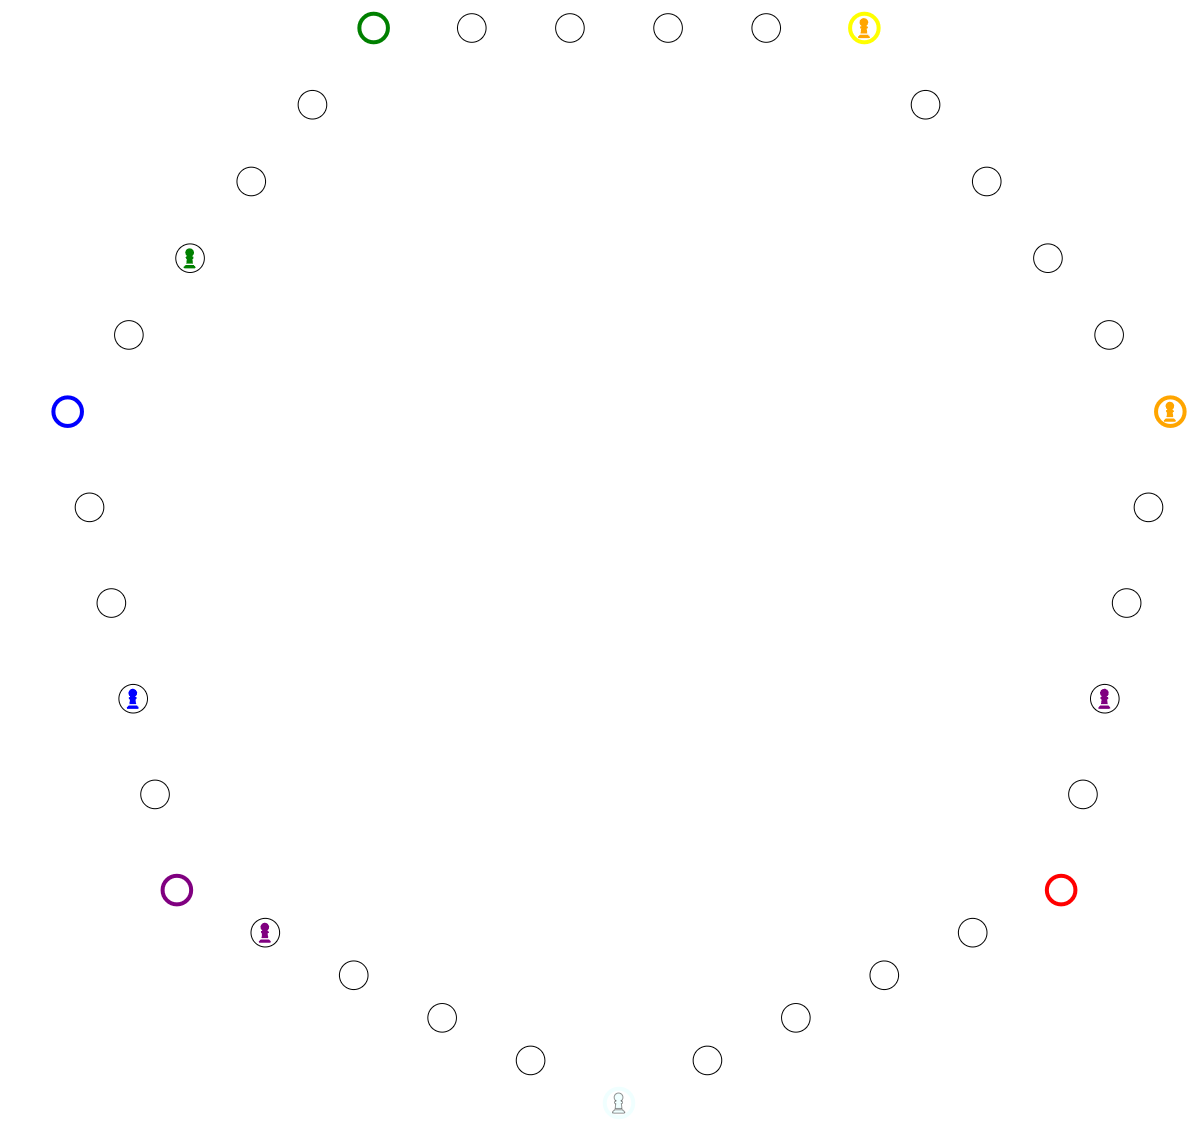
\includegraphics[scale=0.5]{7espalya}
\end{figure}



Miután kirajzoltam a pályát,a következő feladatom az volt, hogy megjelenítsem a játékosok bábujait a pályán. Ehhez a playingBoard komponens \textit{mounted} életciklusában létrehoztam egy \textit{watch} függvény ami figyeli, hogy az aktuális táblával, amivel éppen játszanak, történik-e valamilyen változás. A Stage objektumból le lehet kérdezni bizonyos típusú objektumokat. Mivel tudom, hogy a mezők mind \textit{Circle} típusú objektumok, így egy tömbbe egyszerűen el tudtam menteni az összes mező objektumot. A \textit{watch} függvényben egy 3-szor egymásba ágyazott for-ciklus szerepel. Első ciklus a mezőken iterál majd a második ciklus a játékosokon, a harmadik pedig az egyes játékos bábujain. Hogyha találok egy olyan bábut, aminek a \textit{positionOnTheBoard} tulajdonsága megegyezik a mező azonosítójával, akkor tudom hogy azon a mezőn kell, hogy legyen bábu. Így ebben az esetben létrehozok egy Konva által nyújtott \textit{Path} objektumot. A \textit{Path} objektumnak a data tulajdonságának meg lehet adni egy svg\footnote{Scalable Vector Graphics}-nek a leírását. Ez azért fontos mert így bármilyen svg-t meg tudok jeleníteni az alkalmazásomban. A projektembe beimportáltam a Font-Awesome könyvtárnak pár ikonját, és a bábu megjelenítéséhez a \textit{faChessPawn} ikonjukat használtam. Ennek az ikonnak az svg leírását ki tudtam nyerni, így meg tudtam jeleníteni ezt az ikont mint objektum, tehát több tulajdonságát is állíthattam, mint a pozíciója, milyen színű legyen az ikon, valamint hogy hol helyezkedjen el. Tehát hogyha találtam egy olyan mezőt aminek az azonosítója megegyezett a bábu \textit{positionOnTheBoard} tulajdonságával, akkor létrehozok egy Path objektumot, és a koordinátáját beállítom, a mező koordinátájára,az azonosítóját a bábu azonosítójára, valamint a színét éppen az adott játékoséra. Mivel az ikon mérete kicsit nagyobb volt mint a mező mérete, így ezt a \textit{scale} tulajdonsággal oldottam meg. Valamint amikor létrehozom az új Path objektumot, egy eseménykezelőt is rakok rá, hogyha rákattintanak, akkor ennek az objektum azonosítójával megegyező bábu lesz a játékos által választott is. 

Ez így sajnos még nem elég a működőképes funkcionalitáshoz. Mivel eddig még csak új objektumokat rajzoltunk ki, viszont ha lépünk egy bábuval, akkor onnan el kell tűnnie, ahonnan elléptünk. Ezt a problémát viszonylag egyszerűen, bár nem túl hatékonyan oldom meg. Mivel amikor változás lép fel a tábla állapotával kapcsolatban, tegyük fel egy bábuval léptek, akkor a tábla új állapotát kapom meg, viszont nem tudom, hogy pontosan mi történt, melyik bábuval léptek. Egy megoldás lenne mindig eltárolni az előző tábla állapotát, és összevetni az újonnan kapottal, viszont egy ilyen kis alkalmazásban egy egyszerűbb megoldás is lehetséges, mégpedig egyszerűen újrarajzolni az egészet. Én az utóbbit választottam. Mielőtt még a 3-szorosan egymásba ágyazott for ciklusba belépnék, és hozzáadnám az új ikonokat az új helyükön, eltávolítom az összes Path objektumot a Stage objektumból. Ezáltal eltűnik a régi tábla állása, és már csak az új állapot szerinti Path objektumokat adjuk hozzá, és így olyan mintha lépne a játékos a bábuval. Mivel ez nagyon gyorsan történik, a felhasználó észre sem veszi, hogy az összes bábu eltűnt majd újra megjelent. Ennek a módszernek az a hátránya, hogy így az összes többi bábut, amivel nem léptek, feleslegesen veszem le, majd teszem vissza ugyan oda a pozícióba, de mivel ez a szám kicsi és nem ront a játékélményben, így inkább ezt az egyszerű megoldást választottam. 

A felhasználói élmény növelése érdekében valahogy meg akartam jeleníteni, hogy az adott játékosnak éppen melyik a kiválasztott bábuja amivel lépni fog. Az éppen kiválasztott bábu egy kis fekete körvonalat kap az ikon köré, így jelezve a felhasználónak, hogy az van kiválasztva (\ref{babu}.ábra).
\begin{figure}
	\caption{Egy kiválasztott bábu megjelenítése}
	\label{babu}
	\centering
	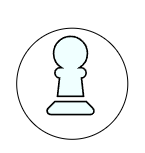
\includegraphics[scale=0.5]{babu}
\end{figure}
\FloatBarrier

 Ennek automatikusan kellett működnie, hiszen ha a robotot bekapcsolja a felhasználó akkor is jelezni kell, hogy melyik bábuval fog éppen lépni a robot. Ehhez is egy \textit{watch} függvényt használtam ami azt nézi, hogy változott-e  a kiválasztott bábu. Amint változik, megkeresi a Stage objektumban azt a objektumot, ami újonnan lett a kiválasztott bábu és a \textit{stroke} valamint \textit{strokeWidth} tulajdonságát beállítja a megfelelőre (\ref{addOutline}.ábra).

\begin{figure}
	\caption{A körvonal beállítása az aktuális bábura}
	\begin{minipage}{\textwidth}
		\begin{lstlisting}[style=javascriptStyle]
			 watch(() => gamePlayStore.selectedPiece, (selectedpiece) => {
				let paths = stage.find("Path");
				removeEveryOutline(paths);
				let selectedPiece = findPieceInStage(selectedpiece);
				if (selectedPiece) {
					selectedPiece.stroke('black');
					selectedPiece.strokeWidth(10);
				}
			})
			\end{lstlisting}
		\end{minipage}
		
		\label{addOutline}
	\end{figure}
	\FloatBarrier

 Itt is hasonló problémába ütközünk mint a lépés megvalósításánál, hiszen ez a függvény mindig csak beállítja a tulajdonságot, sosem veszi le, ha már éppen nem az a választott bábu, ami akkor történhet ha a felhasználó egy másik bábura kattintott, vagy már egy másik játékos van soron. A megoldás is hasonló mint a lépés implementálásánál: eltüntetjük a körvonalat az összes ikonról, arról is amin nem volt, majd beállítjuk az aktuálisra (\ref{removeOutline}.ábra). Ez is felesleges munkát végez de mivel szemmel láthatólag nem ront a felhasználói élményen, így benne hagytam. 
\begin{figure}
	\caption{Az összes körvonal eltávolítása a Path objektumokról}
	\begin{minipage}{\textwidth}
		\begin{lstlisting}[style=javascriptStyle]
		function removePathsFromLayer(layer) {
			const children = layer.getChildren(); // Get all children of the layer
			for (let i = children.length - 1; i >= 0; i--) {
				const child = children[i];
				if (child instanceof Konva.Path) {
					child.destroy(); // Remove the Konva.Path object
				}
			}
			layer.draw(); // Redraw the layer to apply the changes
		}
		\end{lstlisting}
	\end{minipage}
	
	\label{removeOutline}
\end{figure}




\subsubsection{Többjátékos mód}
A többjátékos módot az SSE eseményekre való feliratkozással oldottam meg. Magát a több játékos módot úgy teszteltem, hogy egyszerre több lapon nyitottam meg a böngészőmben a
kliens alkalmazást, és játszottam 2 játékos személyében. 

Első feladat volt felépíteni a kapcsolatot a backenden lévő SseEmitterrel. Ez javascriptben nagyon egyszerűen megvalósítható, csak egy új \textit{EventSource} objektumot kellett létrehozni, aminek paraméterében a backenden lévő elérési utat kellett megadni, ami esetünkben \textbf{"http://localhost:8080/subscribe"} volt. Amint létrejön a \textit{new} kulcsszóval az objektum, már fel is építi a kapcsolatot automatikusan, nem kell vele több mindent csinálni. Így ezt a lépést rögtön az alkalmazás elején megtettem, az eseményekre csak később iratkoztam fel, amikor már releváns volt. Az eseménykezeléssel foglalkozó fájlokat egy külön mappába helyeztem el, mivel így strukturált maradt az alkalmazás.
Először a Board komponensen belül iratkoztam fel a PlayerChange és StatusChange eseményekre. Ezek akkor sülnek el, amikor egy tábla státusza megváltozik, vagy egy játékos fel- vagy lejelentkezik egy játékra. Az eseményekre való feliratkozást és kezelését két külön fájlban csináltam, mivel így tisztább, és könnyebben olvasható a kód. Pinia store-ban tároltam el az EventSource objektumot amit létrehoztam a kapcsolat kialakításához, hogy ehhez globálisan hozzáférhessek. A feliratkozást az \textit{addEventListener} függvénnyel végeztem el, itt kellett megadni az esemény nevét is, amit majd figyelni. Paraméterben mindig átadtam az a táblának az azonosítóját, amire éppen kíváncsiak vagyunk, így el tudtuk magunkat szeparálni azoktól a tábláktól amikkel esetleg más játékosok játszanak. Itt kellett definiálni, azt is, hogyha megtörténik az esemény akkor mit csináljon az alkalmazás (\ref{statuschange}.ábra). Ezeket a függvényeket rendszereztem egy külön fájlba, hogy átláthatóbb legyen az alkalmazás. Figyelni kellett arra is, hogyha nem éppen az adott felhasználó által csatlakoztatott játékos van soron, akkor a Roll és Move gombokat le kellett tiltani, hogy még véletlenül se tudjon egy másik felhasználó helyett dobni vagy lépni. 
\begin{figure}
	\caption{A StatusChange eseményre való feliratkozás és kezelése}
		\begin{minipage}{\textwidth}
			\begin{lstlisting}[style=javascriptStyle]
				async function initStatusChange(board) {
					const boardStore = useBoardStore();
					boardStore.eventSource.addEventListener("StatusChange" + board.id, async function (event) {
						let newStatus = JSON.parse(event.data);
						await handleStatusChange(newStatus);
					})
				}
			\end{lstlisting}
		\end{minipage}
		\begin{minipage}{\textwidth}
			\begin{lstlisting}[style=javascriptStyle]
				async function handleStatusChange(statusChangeMessage) {
					const boardStore = boardStoreFactory();
					const gamePlayStore = gamePlayStoreFactory();
					if (statusChangeMessage.newStatus === "FINISHED") {
						await handleFinished(boardStore,gamePlayStore,statusChangeMessage);
					}
					else if (statusChangeMessage.newStatus === "STARTED" && boardStore.joinedPlayer.length > 0) {
						await handleStarted(boardStore,gamePlayStore,statusChangeMessage)
					}
					else if (statusChangeMessage.newStatus === "CREATED") {
						await handleCreated(boardStore,statusChangeMessage)
					}
				}
			\end{lstlisting}
		\end{minipage}
	\label{statuschange}
\end{figure}

A PlayerChange esemény lekezelése viszonylag egyszerű volt. A szerver elküldte a megváltozott tábla új állapotát, majd kicseréltem a \textit{boards} tömbben arra az elemről, ami még erről a tábláról a régi állapotát tartalmazta. Mivel azt a folyamatot, hogy kicserélek egy táblát a \textit{boards} tömbben egy újra, nagyon sokszor megcsinálom, ezért írtam rá egy külön függvényt. 

A StatusChange esemény implementálása kicsit összetettebb volt. Attól függően hogy milyen állapotba került a tábla, különböző dolgokat kellett csinálni. Hogyha CREATED státuszba került, akkor ellenőrizni kellett, hogy újonnan létrehozott tábla, vagy csak egy táblát Reseteltek, és így került ilyen státuszba. Ha az előbbi történt akkor csak hozzá kellett adni a létrehozott táblát a \textit{boards} tömbhöz, ha az utóbbi, akkor ki kellett cserélni a tömbben.Mivel a StatusChange összes eseményét megkapom, hiszen minden tábláról tudni akarom, hogy éppen milyen állapotban van, így ennek az eseménynek a kezelése több körültekintést igényel. Ha a STARTED állapotba kerül a tábla, akkor nem tudjuk hogy ki indította el. Így hogyha arra a táblára mi is csatlakoztunk, akkor minket is arra a nézetre kell, hogy navigáljon az alkalmazás ahol maga a játék történik. Így el kell tárolnom a \textit{player} objektumokat amikkel csatlakoztam a táblához, és hogyha azon a táblán rajta vagyunk, amit elindítottak, akkor átnavigál a másik nézetre az alkalmazás. Egyébként pedig csak frissíti a \textit{boards} tömböt az új táblával. Hogyha FINISHED státuszba kerül a tábla, hasonlóan járunk el mint előzőleg. Hogyha vannak csatlakozott játékosaink a táblán, akkor átnavigál minket a játék eredmény nézetre, egyébként pedig frissíti a \textit{boards} tömböt. 

A RollChange és a PositionChange eseményekre akkor iratkoztam fel, amikor a \textit{playing} nézetre navigált az alkalmazás. Itt már csak azokat az eseményeket kapjuk el, amik éppen az adott táblához tartoznak, tehát két egyszerre folyó játék nem zavarja meg egymást. A RollChange esemény elküldi, hogy hányast dobott az adott játékos. Ha ez egy olyan szám amivel nem tud lépni az adott játékos, akkor rögtön egy PositionChange esemény is érkezik, ami a tábla új állapotát adja meg. Ez az állapot csak abban különbözik az előzőtől, hogy a soron következő játékos azonosítója megváltozik. Mivel ez is egy Store-ban lévő változó, a felület rögtön frissül, amint ez megváltozik, így amint már nem tud lépni a játékos, rögtön a következő játékost írja ki a felület, mint soron következő. Hogyha tud lépni vele, akkor a Move gomb megnyomása után érkezik a PositionChange esemény, ami tartalmazza a bábu új helyzetét. Hogyha hatost dobott a játékos, tehát megint ő jön, akkor a soron következő játékos azonosítója nem változik az üzenetben.  

A játék végén fontos, hogy a kapcsolatot megszüntessük a backend szerverrel, mivel amint visszanavigálunk a kezdő oldalra, hogyha megmaradnának az előző játékból maradt eseménykezelőink, akkor esetleg olyan táblának az eseményeire is fel lehetnénk iratkozva, egy új játék alatt, amit nem is mi indítottunk el. Ezt az \textit{evenSource.close} függvénnyel tehetjük meg. Valamint itt a Pinia Store-okat is alaphelyzetbe állítom, hiszen sok állapotot őriztünk meg az előző játékból, amikre már nincsen szükségünk. Ezek az utasítások (\ref{reset}.ábra) az Ok gombra vannak kötve az eredménytábla alján. Ilyenkor visszanavigálunk a kezdő nézetre ahol újra létrehozzuk a kapcsolatot az SSE Emitterrel valamint feliratkozunk a PlayerChange és StatusChange eseményekre.  
\begin{figure}
	\caption{SSE kapcsolat megszüntetése, és a store-ok alaphelyzetbe állítása}
	\begin{minipage}{\textwidth}
		\begin{lstlisting}[style=javascriptStyle]
			function closeScoreboard(router){
				const gameStore = useGamePlayStore();
				const boardStore = useBoardStore();
				boardStore.eventSource.close();
				boardStore.$reset();
				gameStore.$reset();
				router.push({
					path: '/boardManagement',
				});
				
			}
		\end{lstlisting}
	\end{minipage}
	
	\label{reset}
\end{figure}
\FloatBarrier
\subsubsection{Robot}
Egy robotot is implementáltam a felhasználóknak, amit hogyha bekapcsolunk akkor helyettünk játszik. Be lehet állítani, hogy pontosan milyen erősségű robotot akarunk szimulálni, van \textit{Beginner} \textit{Intermidiate} és \textit{Advanced}, mindegyik kicsit jobb az előzőnél. Hogyha beállítjuk, hogy a robot játsszon helyettünk, akkor a Roll és a Move gombokat nem lehet használni. Bármikor a játék folyamán be lehet állítani, hogy a robot vegye át az irányítást, valamint azt is hogyha ki szeretnénk kapcsolni. Egy leugró ablakban kell kiválasztani, hogy melyik stratégiát szeretnénk választani, alapértelmezett a \textit{Beginner}. Ennek az implementálásához, eléggé kézenfekvő módon a Strategy pattern-t alkalmaztam. Ez egy olyan programtervezési minta, amit olyan esetekben szokták használni, hogyha egy bizonyos algoritmust akarunk változtatni a környezettől függően. A mintában van egy interfész amit, a különböző stratégiák megvalósítanak, és implementálják le különféle módokon, majd ezt az interfészt használva tudjuk alkalmazni az algoritmusokat. A Pinia Store-ban definiáltam egy robotStrategy függvényt és ezt állítottam be, attól függően hogy mit állított be a felhasználó. Majd létrehoztam egy \textit{executeRobotStrategy} függvényt ami csak meghívja az előbb beállított metódust. Létrehoztam egy komponenst, ami egy legördülő menüből állt, és a választott értékének függvényében állítottam be a megfelelő stratégiát (\ref{setStrat}.ábra) A komponens \textit{mounted} életciklusában beállítottam alapértelmezettként, hogy Beginner stratégiát alkalmazzon.

\begin{figure}
	\caption{Egyes stratégiák beállítása a kiválasztott érték függvénynében}
	\begin{minipage}{\textwidth}
		\begin{lstlisting}[style=javascriptStyle]
			watch(selectedStartegy,(newValue) => {
				if(newValue === "Intermidiate") gamePlayStore.setRobotStartegyToIntermidiate();
				else if(newValue === "Advanced") gamePlayStore.setRobotStartegyToAdvanced();
				else gamePlayStore.setRobotStartegyToBeginner();
			})
			onMounted(()=> {
				gamePlayStore.setRobotStartegyToBeginner();
			})
		\end{lstlisting}
	\end{minipage}
	
	\label{setStrat}
\end{figure}
\FloatBarrier
Miután kiválasztottuk a stratégiát és rányomunk a checkboxra, a robot folytatja a játékot helyettünk. Létrehoztam egy \textit{watch} függvényt ami figyeli a checkbox értékét, és annak függvényeben hívja meg a \textit{robotStep} metódust. Itt zajlik le a kockadobás és a bábu mozgatása is. Itt igazából csak azokat a függvényeket hívom meg amik eddig a Roll és Move gombokra voltak kötve egymás után, így szimulálja az emberi inputot. Egy ilyen \textit{robotStep} függvény lefutása egy Roll és Move gomb megnyomással egyenértékű. Mivel amikor a saját bábuval lépünk, akkor is kapunk eseményt, hogy a pálya állapota megváltozott, így a \textit{handlePositionChange} függvényben is meghívtam a \textit{robotStep} függvényt. Így folyamatosan fog lépni a robot nem kell a felhasználónak semmit sem csinálnia. Így akkor is meghívódik a \textit{robotStep} függvény amikor egy más játékos lépett, hiszen akkor kapunk PositionChange eseményt, de mivel ellenőrzöm, hogy csak akkor fusson le a \textit{rollDice} és a \textit{movePlayer} függvény, ha éppen a mi játékosunk van soron, így ez nem okoz problémát a működésben. A függvény belsejében a program lefutását kicsit lassítom a \textit{setTimeout} függvénnyel, ami a futó szálat alvó állapotba helyezi. Hogyha ezt a lépést nem tenném meg akkor a robot lépései túl gyorsak lennének a felhasználóknak, hogy felfoghassák mi is történik a pályán. Ezt az értéket 350  milliszekundumra állítottam. Ellenőrizni kell, hogy az éppen soron következő játékost éppen az adott felhasználó csatlakoztatta-e fel, hiszen ha ezt nem ellenőriznénk akkor hogyha egy felhasználó is bekapcsolja a robotot, az mindenki helyett lépni fog. Mielőtt a mozgást elvégző http kérést elküldenénk, meghívjuk a Strategy minta alapján készült "interfészünket" ami az \textit{executeStrategy} függvény. A stratégiák lényegében csak egy dolgot csinálnak: beállítják, hogy melyik legyen az a bábu amivel majd lépni fogunk. Gyakorlatilag a játékban itt van gondolkodni valónk, hiszen sajnos azt, hogy hányast dobjunk, nem tudjuk befolyásolni.A \textit{Beginner} stratégiájú robot nem csinál semmit, mindig csak ugyanazzal a bábuval akar beérni a célba , ha ez sikerül akkor megy a következőre. Az \textit{Intermidiate} robot már kihasználja a hatosok adta lehetőségeket. Hogyha a felhasználó hatost dob akkor lerak egy új bábut a táblára. Ha nem hatost dobott a felhasználó, akkor megkeresi azt a bábut, ami legközelebb áll ahhoz hogy beérjen, és azt választja ki. A legközelebbi bábu kiválasztása bonyolultabb, mint ahogyan hangzik. Mivel körbe megy a tábla ezért hogyha a kezdő pozíciója a játékosnak 0, akkor a hozzá legközelebbi mező, ahonnan a bábuk be tudnak érni, az értéke a legnagyobb szám lesz, hiszen pont azelőtt a mező előtt ér véget a kör. Viszont a többi kezdőpozíciója előtt már "újrakezdődött" a számolás, így nem elég csak azt megnézni, hogy melyik a legnagyobb szám és azt kiválasztani. A \textit{findClosestPiece} függvény, ami meghatározza a legközelebbi bábut a beéréshez, először is minden táblán lévő bábu helyzetéből kivonja, a játékos kezdő pozícióját és ezeket a pozíciókat eltárolja egy tömbbe (\ref{absPos}.ábra).
\begin{figure}
	\caption{A kiinduló helytől számított relatív pozíciók kiszámítása}
	\begin{minipage}{\textwidth}
		\begin{lstlisting}[style=javascriptStyle]
			getRelativPosition(){
				let positionContainer = [];
				this.currentPlayer.pieces.forEach(piece => {
					if(piece.positionOnTheBoard >=0)
					{
						let absolutePosition = piece.positionOnTheBoard - this.currentPlayer.startingIndexOnBoard;
						positionContainer.push({absolutePos: absolutePosition,piece:piece});
						
					}
				})
				return positionContainer;
			},
		\end{lstlisting}
	\end{minipage}
	
	\label{absPos}
\end{figure}
\FloatBarrier
 A negatív és pozitív értékű pozíciókat szétválogatja két különböző tömbbe. Mivel ha negatív értékű a pozíció akkor az biztosan közelebb van a bejutáshoz, mint a pozitív, így először ezen a tömbbön iterál végig. Itt minél nagyobb a negatív érték, annál közelebb van a beéréshez, így rendezi nagyság szerint, és így megkapjuk a legközelebbi pozíciót. Ha esetleg nincsen negatív értékű pozíció, akkor ugyanezt megcsináljuk a pozitív értékűekre (\ref{findClos}.ábra). 

\begin{figure}
	\caption{findClosestPiece függvény implementálása}
	\begin{minipage}{\textwidth}
		\begin{lstlisting}[style=javascriptStyle]
		findClosestPiece(){
			let absolutePos = this.getAbsolutePositions();
			let negativPos = absolutePos.filter(p=>p.absolutePos<0);
			let positivePos = absolutePos.filter(p=>p.absolutePos>=0);
			if(negativPos.length > 0) {
				const closest = negativPos.reduce((max, current) => (current.absolutePos > max.absolutePos ? current : max), negativPos[0]);
				this.selectedPiece = closest.piece;
			}
			else if(positivePos.length > 0){
				const closest = positivePos.reduce((max, current) => (current.absolutePos > max.absolutePos ? current : max), positivePos[0]);
				this.selectedPiece = closest.piece;
			}
		},
		\end{lstlisting}
	\end{minipage}
	
	\label{findClos}
\end{figure}
\FloatBarrier
 Az \textit{Advanced} robot pedig használja azt a szabályát a játéknak, hogyha egy bábu olyan mezőre lép ahol éppen áll egy másik játékos bábuja, akkor azt leüti a tábláról, így újra csak hatossal lehet visszatenni a játékba. Így először azt ellenőrzi, hogy tud e úgy lépni valamelyik bábuval, amivel le tudna ütni egy másikat, ha ez nem lehetséges, akkor használja az \textit{Intermidiate} stratégiát.
 
A két stratégiát teszteltem egy sima \textit{Beginner} robot ellen egy kétszemélyes, 10 mezőt tartalmazó pályán. Minden játékosnak 5 darab bábuja volt. 10 darab játszmát szimuláltam le. Az \textit{Intermidiate} mind az \textit{Advanced} stratégia 7 darab győzelmet szerzett. Ez arra enged következtetni, hogy \textit{Intermidiate} stratégiában implementált logika segíti a felhasználót a nyerésben, hiszen kihasználja a játék egyes szabályait, viszont nem olyan nagy mértékben, mint ahogy remélnénk. Az \textit{Advanced} stratégia az eredményekben nem mutatott javulást, viszont ez fogható a kis játéktérre, hiszen egy nagyobb pályán, több játékossal játszva, a leütést nagyobb eséllyel tudta volna használni. 
\section{Összefoglalás}
\subsection{Továbbfejlesztési lehetőségek}
Az alkalmazást többféleképpen lehetne tovább fejleszteni. Egyrészt újabb funkciókat lehetne belevinni, mint például egy bajnokság indítása bizonyos időközönként, vagy egy másfajta módban indítani a játékot, ahol a hagyományostól eltérő szabályok vannak életben. A bejelentkezett felhasználóknak a preferált beállításait el lehetne menteni, vagy esetleg az eddigi meccseit számon tartani. Valamint természetesen, hogy ne csak lokálisan futtatható legyen a játék, hanem az interneten elérhető weboldalak valamelyikére feltölteni, vagy egy saját szerveren futtatni, hogy másokkal is játszhassuk a társast. 
\subsection{Tapasztalatok}
A társasjáték fejlesztése során rengeteg gyakorlati tapasztalatot szereztem a webalkalmazások készítésével kapcsolatban. Jobban megismertem a böngészők működését, és hogy hogyan segíthetik a fejlesztőket. Sokat fejlődtem abban, hogy hogyan kell megtervezni a backend részét az alkalmazásnak, valamint az autentikációt integrálni, hogy csak a bejelentkezett felhasználók tudjanak hozzáférni az erőforrásokhoz. A http kommunikációról egy magabiztos tudást szereztem, aminek igen nagy haszna van a későbbi karrieremre tekintve. Összességében sikerült elvégeznem a kitűzött céljaimat, és elégedett vagyok a létrehozott alkalmazással.


\newpage
\bibliographystyle{plain} % We choose the "plain" reference style
\bibliography{refs} % Entries are in the refs.bib file

\end{document}